\documentclass[letterpaper]{article} % DO NOT CHANGE THIS
% \usepackage[submission]{aaai25}
 \pdfoutput=1 
\usepackage{aaai25}
\usepackage{aaai25}  % DO NOT CHANGE THIS
\usepackage{times}  % DO NOT CHANGE THIS
\usepackage{helvet}  % DO NOT CHANGE THIS
\usepackage{courier}  % DO NOT CHANGE THIS
\usepackage[hyphens]{url}  % DO NOT CHANGE THIS
\usepackage{graphicx} % DO NOT CHANGE THIS
\urlstyle{rm} % DO NOT CHANGE THIS
\def\UrlFont{\rm}  % DO NOT CHANGE THIS
\usepackage{natbib}  % DO NOT CHANGE THIS AND DO NOT ADD ANY OPTIONS TO IT
\usepackage{caption} % DO NOT CHANGE THIS AND DO NOT ADD ANY OPTIONS TO IT
\frenchspacing  % DO NOT CHANGE THIS
\setlength{\pdfpagewidth}{8.5in}  % DO NOT CHANGE THIS
\setlength{\pdfpageheight}{11in}  % DO NOT CHANGE THIS

% notation
\newcommand{\adv}{\operatornamewithlimits{adv}}
\newcommand{\dx}{\text{d}\mathbf{x}_t}
\newcommand{\dy}{\text{d}\mathbf{x}_t^{\adv}}
\newcommand{\trac}{\operatornamewithlimits{trace}}


\newcommand{\diffforward}[2]{
    \STATE{$\mathbf{x}^{#1}_t = \sqrt{\bar{\alpha}_t} \mathbf{x}^{#1} + \sqrt{1-\bar{\alpha}_t} \epsilon_{#2}$}
}
\newcommand{\normaldist}{\mathcal{N}(\mathbf{0}, \mathbf{I})}
\newcommand{\sign}{\operatornamewithlimits{sign}}
\newcommand{\argmin}{\operatornamewithlimits{argmin}}

\newcommand {\first}[1]{\textbf{#1}}
\newcommand {\second}[1]{\underline{#1}}

\usepackage[utf8]{inputenc}
\usepackage[T1]{fontenc}

\usepackage[lines=3]{lettrine}
\usepackage{style/Zallman}
\usepackage[nopatch=footnote]{microtype}
\usepackage{fontawesome}
\usepackage{dsfont}
\usepackage{lmodern}
\usepackage{anyfontsize}
\usepackage{verbatim}
\usepackage{pifont}

\usepackage{quoting}
\usepackage{xcolor}

\usepackage{url}

\usepackage{tcolorbox}
\usepackage{booktabs,array}
\usepackage{makecell}
\usepackage{multirow}
\usepackage{tikz}
\usetikzlibrary{shapes.geometric,positioning}
\usepackage{pgfornament}


\usepackage[frozencache,cachedir=minted-output]{minted}

\usepackage{amsfonts,amssymb,amsmath}
\usepackage[noabbrev,nameinlink,capitalise,compress]{cleveref}
\usepackage{mathtools}
\usepackage{bm}
\usepackage{mathabx}
\usepackage{thmtools,thm-restate}
\usepackage{resizegather}
\usepackage{nicefrac}
\usepackage{xfrac}

\usepackage{enumitem}
\usepackage{setspace}
\usepackage{regexpatch}


% These are are recommended to typeset listings but not required. See the subsubsection on listing. Remove this block if you don't have listings in your paper.
\usepackage{newfloat}
\usepackage{listings}
\DeclareCaptionStyle{ruled}{labelfont=normalfont,labelsep=colon,strut=off} % DO NOT CHANGE THIS
\lstset{%
	basicstyle={\footnotesize\ttfamily},% footnotesize acceptable for monospace
	numbers=left,numberstyle=\footnotesize,xleftmargin=2em,% show line numbers, remove this entire line if you don't want the numbers.
	aboveskip=0pt,belowskip=0pt,%
	showstringspaces=false,tabsize=2,breaklines=true}
\floatstyle{ruled}
\newfloat{listing}{tb}{lst}{}
\floatname{listing}{Listing}
%
% Keep the \pdfinfo as shown here. There's no need
% for you to add the /Title and /Author tags.
\pdfinfo{
/TemplateVersion (2025.1)
}

% DISALLOWED PACKAGES
% \usepackage{authblk} -- This package is specifically forbidden
% \usepackage{balance} -- This package is specifically forbidden
% \usepackage{color (if used in text)
% \usepackage{CJK} -- This package is specifically forbidden
% \usepackage{float} -- This package is specifically forbidden
% \usepackage{flushend} -- This package is specifically forbidden
% \usepackage{fontenc} -- This package is specifically forbidden
% \usepackage{fullpage} -- This package is specifically forbidden
% \usepackage{geometry} -- This package is specifically forbidden
% \usepackage{grffile} -- This package is specifically forbidden
% \usepackage{hyperref} -- This package is specifically forbidden
% \usepackage{navigator} -- This package is specifically forbidden
% (or any other package that embeds links such as navigator or hyperref)
% \indentfirst} -- This package is specifically forbidden
% \layout} -- This package is specifically forbidden
% \multicol} -- This package is specifically forbidden
% \nameref} -- This package is specifically forbidden
% \usepackage{savetrees} -- This package is specifically forbidden
% \usepackage{setspace} -- This package is specifically forbidden
% \usepackage{stfloats} -- This package is specifically forbidden
% \usepackage{tabu} -- This package is specifically forbidden
% \usepackage{titlesec} -- This package is specifically forbidden
% \usepackage{tocbibind} -- This package is specifically forbidden
% \usepackage{ulem} -- This package is specifically forbidden
% \usepackage{wrapfig} -- This package is specifically forbidden
% DISALLOWED COMMANDS
% \nocopyright -- Your paper will not be published if you use this command
% \addtolength -- This command may not be used
% \balance -- This command may not be used
% \baselinestretch -- Your paper will not be published if you use this command
% \clearpage -- No page breaks of any kind may be used for the final version of your paper
% \columnsep -- This command may not be used
% \newpage -- No page breaks of any kind may be used for the final version of your paper
% \pagebreak -- No page breaks of any kind may be used for the final version of your paperr
% \pagestyle -- This command may not be used
% \tiny -- This is not an acceptable font size.
% \vspace{- -- No negative value may be used in proximity of a caption, figure, table, section, subsection, subsubsection, or reference
% \vskip{- -- No negative value may be used to alter spacing above or below a caption, figure, table, section, subsection, subsubsection, or reference

\setcounter{secnumdepth}{2} %May be changed to 1 or 2 if section numbers are desired.

\title{Pixel Is Not A Barrier: An Effective Evasion Attack for Pixel-Domain Diffusion Models}
\author{
%     %Authors
    Chun-Yen Shih\textsuperscript{\rm 1 \rm 2}\equalcontrib, 
    Li-Xuan Peng\textsuperscript{\rm 2}\equalcontrib,
    Jia-Wei Liao\textsuperscript{\rm 1 \rm 2},
    Ernie Chu\textsuperscript{\rm 2}, \\
    Cheng-Fu Chou\textsuperscript{\rm 1},
    Jun-Cheng Chen\textsuperscript{\rm 2}
}

\affiliations{
    %Afiliations
    \textsuperscript{\rm 1} National Taiwan University, \\
    \textsuperscript{\rm 2} Research Center for Information Technology Innovation, Academia Sinica \\
    % If you have multiple authors and multiple affiliations
    % use superscripts in text and roman font to identify them.
    % For example,

    % Sunil Issar\textsuperscript{\rm 2}, 
    % J. Scott Penberthy\textsuperscript{\rm 3}, 
    % George Ferguson\textsuperscript{\rm 4},
    % Hans Guesgen\textsuperscript{\rm 5}
    % Note that the comma should be placed after the superscript

    % 1101 Pennsylvania Ave, NW Suite 300\\
    % Washington, DC 20004 USA\\
    % email address must be in roman text type, not monospace or sans serif
    % proceedings-questions@aaai.org
%
% See more examples next
}

%Example, Single Author, ->> remove \iffalse,\fi and place them surrounding AAAI title to use it
\iffalse
\title{My Publication Title --- Single Author}
\author {
    Author Name
}
\affiliations{
    Affiliation\\
    Affiliation Line 2\\
    name@example.com
}
\fi

\iffalse
%Example, Multiple Authors, ->> remove \iffalse,\fi and place them surrounding AAAI title to use it
\title{My Publication Title --- Multiple Authors}
\author {
    % Authors
    First Author Name\textsuperscript{\rm 1,\rm 2},
    Second Author Name\textsuperscript{\rm 2},
    Third Author Name\textsuperscript{\rm 1}
}
\affiliations {
    % Affiliations
    \textsuperscript{\rm 1}Affiliation 1\\
    \textsuperscript{\rm 2}Affiliation 2\\
    firstAuthor@affiliation1.com, secondAuthor@affilation2.com, thirdAuthor@affiliation1.com
}
\fi


% REMOVE THIS: bibentry
% This is only needed to show inline citations in the guidelines document. You should not need it and can safely delete it.
\usepackage{bibentry}
% END REMOVE bibentry

\begin{document}

\maketitle
\begin{abstract}
Diffusion Models have emerged as powerful generative models for high-quality image synthesis, with many subsequent image editing techniques based on them. However, the ease of text-based image editing introduces significant risks, such as malicious editing for scams or intellectual property infringement. Previous works have attempted to safeguard images from diffusion-based editing by adding imperceptible perturbations. These methods are costly and specifically target prevalent Latent Diffusion Models (LDMs), while Pixel-domain Diffusion Models (PDMs) remain largely unexplored and robust against such attacks. Our work addresses this gap by proposing a novel attacking framework with a feature representation attack loss that exploits vulnerabilities in denoising UNets and a latent optimization strategy to enhance the naturalness of protected images. Extensive experiments demonstrate the effectiveness of our approach in attacking dominant PDM-based editing methods (e.g., SDEdit) while maintaining reasonable protection fidelity and robustness against common defense methods. Additionally, our framework is extensible to LDMs, achieving comparable performance to existing approaches.
\end{abstract}

\section{Introduction}
%
Large Transformers have enabled a number of breakthrough advances in modeling language, vision, audio, biology and numerous other domains \citep{vaswani2017attention}, \citep{dosovitskiy2020image}, \citep{radford2022robust}, \citep{cramer2021alphafold2}. Much of the success of Transformers, powered by the attention operator \citep{vaswani2017attention}, relies on their scaling properties \citep{hoffmann2022training} and the emergence of in-context learning \citep{garg2022can}, which allows them to generalize to unseen data and tasks given context as input. 
%
The Transformer block is a powerful tool for sequence modeling, but it is not without its limitations. One of the most notable is the computational cost, which grows rapidly as the length of the input sequence increases. Specifically, the cost scales quadratically with the length $L$ of the sequence, which places a strict limit on the amount of context that can be considered by the model.
%
Breaking the quadratic barrier is a key step towards new possibilities for deep learning, such as using entire textbooks as context, generating long-form music or processing gigapixel scale images.

Efforts to reduce the computational cost of attention in models primarily involve the use of linearized, low-rank, and sparse approximations \citep{child2019generating,wang2020linformer,kitaev2020reformer,zhai2021attention,roy2021efficient,schlag2021linear,tu2022maxvit}. These approaches introduce a trade-off between expressivity and speed, requiring hybridization with standard attention layers to reach Transformer quality \citep{mehta2022long,dao2022hungry}.

A growing amount of evidence suggests that attention mechanisms only utilize a small portion of their quadratic capabilities for language processing \citep{olsson2022context, dao2022hungry}, leading us to question its role as the gold-standard operator for deep learning at scale. Specifically, we ask:

%
\begin{figure*}[t]
    \centering
    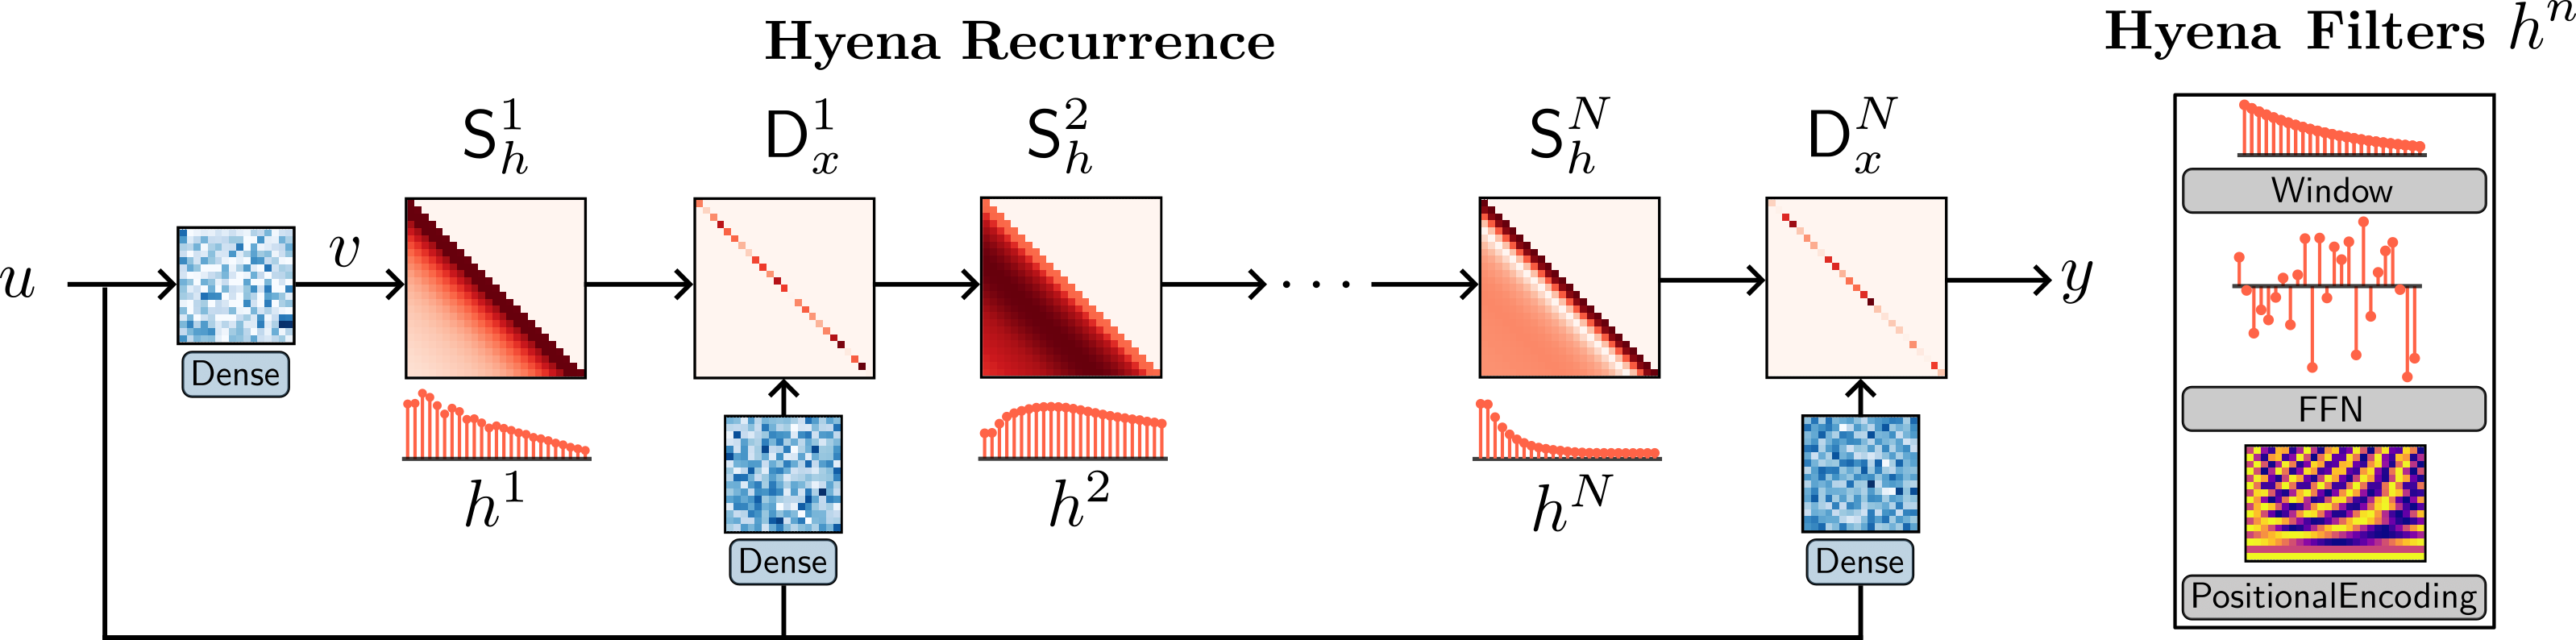
\includegraphics[width=\linewidth]{figures/hyena.png}
    \vspace{-2mm}
    \caption{The ${\sf Hyena}$ operator is defined as a recurrence of two efficient subquadratic primitives: an implicit long convolution $h$ (i.e. {\sf Hyena} filters parameterized by a feed-forward network) and multiplicative element-wise gating of the (projected) input. The depth of the recurrence specifies the size of the operator. {\sf Hyena} can equivalently be expressed as a multiplication with \textit{data-controlled} (conditioned by the input $u$) diagonal matrices $\sD_x$ and Toeplitz matrices $\sS_h$. In addition, {\sf Hyena} exhibits sublinear parameter scaling (in sequence length) and unrestricted context, similar to attention, while having lower time complexity.}
    \label{arch}
\end{figure*}
%

{\centering
\textit{Are there subquadratic operators that can match the quality of attention at scale?}\par}

\vspace{0.5cm}
% 

We obtain a positive answer based on a composition of efficient subquadratic primitives, such as \textit{element-wise multiplication} (gating) and \textit{long convolutions} i.e., convolutions with filter sizes as long as the input. We rely on a set of targeted reasoning tasks, grounded in recent work on \textit{mechanistic interpretability} \citep{elhage2021mathematical,power2022grokking,olsson2022context,zhang2022unveiling} such as recall and induction, to distill three properties of attention correlated with its performance and the quality gap with existing subquadratic approaches: 
%
\begin{itemize}[leftmargin=0.1in]
    \item[$a.$] \textbf{Data control:} Attention implements an expressive \textit{data-controlled} \citep{massaroli2020dissecting} linear operator\footnote{Self-attention can be expressed as $y = \sA(k, q) v$ where $\sA$ is the \textit{attention matrix} conditioned by linear projections $k, q$ of the input and multiplied by $v$, another projection.}, encoding an entire family of linear functions in a single block.
    \item[$b.$] \textbf{Sublinear parameter scaling:} Parameter counts of attention layers are decoupled from sequence length, allowing Transformers to allocate more parameters elsewhere e.g., the \textit{feed-forward neural networks} ({$\sf FFN$s}) between attention layers.
    \item[$c.$] \textbf{Unrestricted context:} For a given input, attention has an unrestricted context i.e., it can approximate dependencies between any two inputs, without arbitrary restrictions such as locality (except in cases using masking such as autoregressive models).
\end{itemize}
%
\paragraph{The ${\sf Hyena}$ hierarchy}
%
Guided by these findings, we introduce the ${\sf Hyena}$ hierarchy, an operator defined by a recurrence of two efficient subquadratic primitives: \textbf{a long convolution and element-wise multiplicative gating} (see Figure \ref{arch}). A specified depth (i.e., number of steps) of the recurrence controls the size of the operator. For short recurrences, existing models are recovered as special cases \citep{mehta2022long,dao2022hungry}. By mapping each step in the ${\sf Hyena}$ recurrence to its corresponding matrix form, we reveal ${\sf Hyena}$ operators to be equivalently defined as a decomposition of a \textit{data-controlled} matrix i.e., a matrix whose entries are functions of the input. Furthermore, we show how ${\sf Hyena}$ operators can be evaluated efficiently without materializing the full matrix, by leveraging fast convolution algorithms \citep{selesnick2017fast}. Empirically, ${\sf Hyena}$ operators are able to significantly shrink the quality gap with attention at scale, reaching similar perplexity and downstream performance with a smaller computational budget (Section \ref{res:lm}) and \textbf{without hybridization} of attention.
%

\paragraph{Narrowing the capabilities gap}
%
The design of {\sf Hyena} is motivated by a quality gap between standard dense attention and alternative subquadratic operators, which we identify by focusing on reasoning tasks correlated with language modeling performance at scale. We extend the suite of basic mechanistic interpretability benchmarks (\textit{induction} and \textit{recall}) with additional tasks that probe how quickly model performance degrades when task complexity increases (e.g. vocabulary size grows). In addition, we investigate the optimal parameterization of long convolutions in ${\sf Hyena}$. In the most challenging settings with hundreds of thousands of tokens, our implicit parameterization scheme improves over other operators leveraging state spaces \citep{gu2021efficiently}, frequency-domain parametrizations \citep{li2020fourier}, or standard convolutions by over $50\%$ accuracy.
%
\paragraph{Scaling in language and vision}
%
Next, we aim to verify whether rankings in our reasoning benchmark suite are predictive of quality at scale. We test ${\sf Hyena}$ on autoregressive language modeling at the sub-billion parameter scale, setting a new state-of-the-art for dense-attention-free architectures in standard datasets ({\sc WikiText103} and {\sc The Pile}) and matching Transformer quality. On the {\sc The Pile} at the $335$M parameter scale, we match Transformer perplexity with a $20\%$ reduction in the total count of \textit{floating point operations} (FLOPs). As an extension, we investigate the generality of ${\sf Hyena}$ operators by testing on large-scale image recognition, replacing attention in the Vision Transformer (ViT) \citep{dosovitskiy2020image}. In image classification, ${\sf Hyena}$ is able to match attention in accuracy when training on ImageNet-1k from scratch.
%
\paragraph{Toward much longer context}
%
Finally, we benchmark the efficiency of ${\sf Hyena}$ on long sequences. We measure $5$x speedups over dense self-attention at length $8192$ -- $2$x over highly optimized FlashAttention\footnote{FlashAttention is already 2-4x faster than a standard attention implementation in PyTorch.} \citep{dao2022flashattention} -- and $100$x speedup over FlashAttention at sequence lengths of $64$k, where standard attention implementation in PyTorch runs out of memory. 
\section{Related Work}
\subsection{Diffusion Model}
%
In the realm of generative models, diffusion models \cite{ho2020denoising, sohl2015deep} have become foundational due to their exceptional ability to produce high-quality and diverse outputs. Initially developed with the U-Net architecture, these models have demonstrated impressive performance in image and video generation \cite{ramesh2022hierarchical, rombach2022high, ho2022video, saharia2022photorealistic, wei2024dreamvideo, wei2024dreamvideo2, wang2023modelscope, chen2023videocrafter1, chen2024videocrafter2}. 
%

However, the scalability of U-Net-based diffusion models is inherently constrained, posing challenges for applications requiring larger model capacities for enhanced performance. To address this limitation, Diffusion transformers (DiT) \cite{peebles2023scalable} represent a significant advancement. By utilizing the scalable architecture of transformers \cite{vaswani2017attention}, DiT provides an effective means to increase model capacity.
%
A notable achievement in this field is the advancement in generating long videos through the large-scale training of Sora \cite{Sora}, which employs a transformer-based Diffusion architecture for comprehensive simulations of the physical world. This underscores the considerable impact of scaling transformer-based Diffusion models.
%
An increasing number of studies have adopted the Diffusion transformer as the noise estimation network~\cite{chen2023pixart, chen2024pixart, Open-Sora, Open-Sora-Plan, ma2024latte, yang2024cogvideox}.

\subsection{Diffusion Model Acceleration}
%
Despite the notable performance of Diffusion models in image and video synthesis, their significant inference costs hinder practical applications. Efforts to accelerate Diffusion model inference fall into two primary categories. First, techniques such as DDIM~\cite{song2020denoising} allow for fewer sampling steps without sacrificing quality. Additional research has focused on efficient ODE or SDE solvers~\cite{song2019generative, jolicoeur2021gotta, lu2022dpm, karras2022elucidating, lu2022dpm++}, using pseudo numerical methods for faster sampling. Second, approaches include distillation~\cite{salimans2022progressive, wang2023videolcm}, quantization~\cite{li2024q, he2024ptqd, so2024temporal, shang2023post}, and distributed inference~\cite{li2024distrifusion} are employed to reduce the workload and inference time.  

However, these methods often demand additional resources for fine-tuning or optimization. Some training-free approaches~\cite{bolya2023token, wang2024attention} streamline the sampling process by reducing input tokens, thereby eliminating redundancy in image synthesis. Other methods reuse intermediate features between successive timesteps to avoid redundant computations~\cite{wimbauer2024cache, so2023frdiff, zhang2024cross}. DeepCache~\cite{xu2018deepcache} and Faster Diffusion~\cite{li2023faster} utilize feature caching to modify the UNet Diffusion, thus enhancing acceleration. FORA~\cite{selvaraju2024fora} and $\triangle$-DiT~\cite{chen2024delta} adapts this mechanism to DiT by caching residuals between attention layers. PAB~\cite{zhao2024real} caches and broadcasts intermediate features at various timestep intervals based on different attention block characteristics for video synthesis. While these methods have improved Diffusion efficiency, enhancements for DiT in visual synthesis remain limited.
\section{Background on Diffusion Models}

Score-based models and diffusion models allow to generate samples starting from easy-to-sample Gaussian noise to complex target distributions via
iteratively applying the score function of learned distribution during sampling, i.e., the gradient of underlying probability distribution $\nabla_{\mathbf{x}} \log p(\mathbf{x})$ with respect to $\mathbf{x}$. However, the exact estimations of the score functions are intractable. 

To bypass this problem, Yang Song et al. proposed slice score matching~\cite{song2020sliced}, and Ho et al. proposed Denoising Diffusion Probability Model (DDPM)~\cite{ho2020denoising} that first gradually perturbs the clean data with linear combinations of Gaussian noise and clean data, as $\mathbf{x}_t = \sqrt{\bar{\alpha}_t} \mathbf{x} + \sqrt{1 - \bar{\alpha}_t} \epsilon_t$ via the predefined timestep schedulers where $t \in[0, T]$ and $\epsilon_t \sim \mathcal{N}(0, \mathbf{I})$, then they finally become isotropic Gaussian noise as time reaches $T$, this is also referred as forward diffusion. The goal is to train a time-dependent neural network that can learn to denoise noisy samples given corresponding timestep $t$. Specifically, the training objective is the expectation over noise estimation MSE, which is formulated as $\mathbb{E}_{t, \mathbf{x}, \epsilon_t}[\| \epsilon_t - \epsilon_{\theta}(\mathbf{x}_t, t) \|_2^2]$, where $\epsilon_{\theta}$ denotes the parametrized neural network, DDPM adopted UNet~\cite{ronneberger2015u} as their noise estimating network. During inference time, we first generate a random Gaussian sample, then iteratively apply the noise estimation network $\epsilon_{\theta}$ and perform denoising operations to generate a new clean sample of the learned distribution. Particularly, Song et.al proposed DDIM~\cite{song2021denoisingdiffusionimplicitmodels} that generalized the DDPM sampling formulation as:

\begin{equation}
    \begin{aligned}
        \mathbf{x}_{t-1} &= \sqrt{\bar{\alpha}_{t - 1}}
        \left(\frac {\mathbf{x}_t - \sqrt{1- \bar{\alpha}_t}\epsilon_{\theta}(\mathbf{x}_t, t)}{\sqrt{\bar{\alpha}_t}}
        \right) \\
        &\quad + \sqrt{1-\bar{\alpha}_{t-1}-\sigma^{2}_t}\epsilon_{\theta}(\mathbf{x}_t, t) + \sigma_t \epsilon_t.
    \end{aligned}
    \label{eq:ddim}
\end{equation}

With $\sigma_t = \sqrt{(1-\bar{\alpha}_{t-1})/(1-\bar{\alpha}_t)} \cdot$ $\sqrt{1-\bar{\alpha}_t /\bar{\alpha}_{t-1} }$, Equation~\ref{eq:ddim} becomes DDPM, and when $\sigma_t = 0$, the sampling process become deterministic as proposed in DDIM since the added noise during each sampling step is null.

\begin{figure}[t]
    \centering
    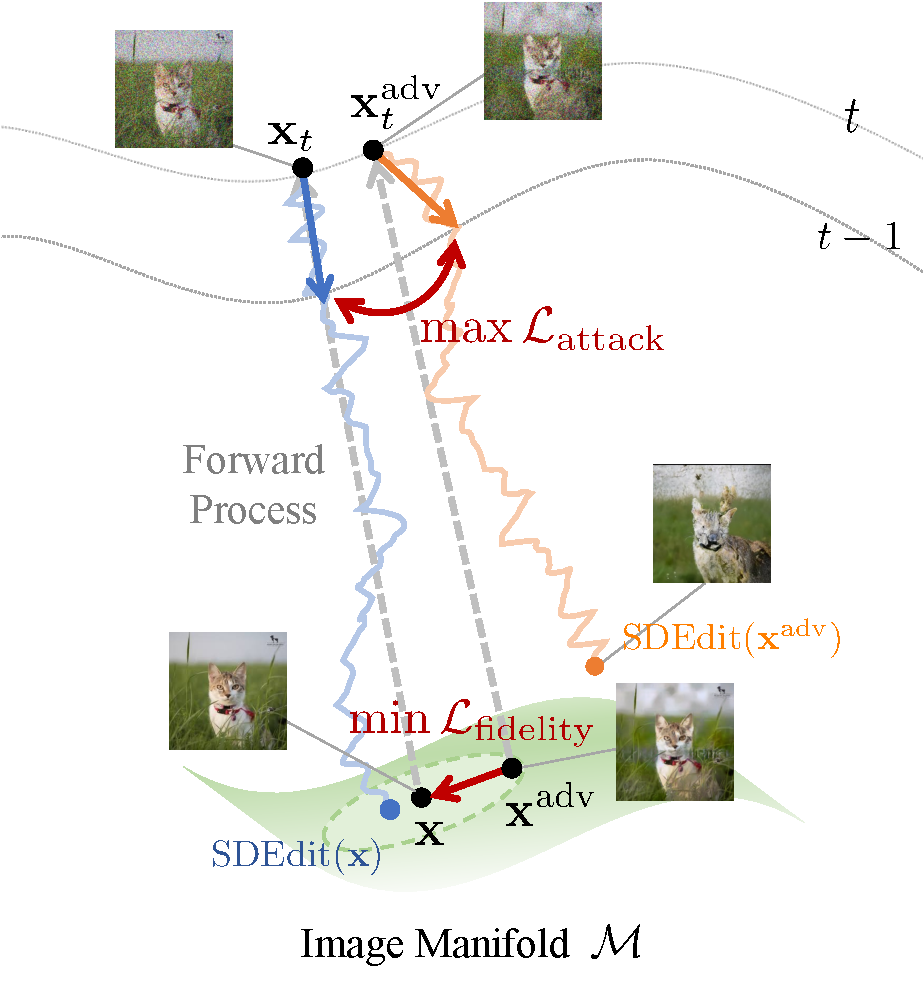
\includegraphics[width=1\linewidth]{figures/manifold.pdf}
    \caption{Conceptual illustration of our method. We randomly forward both the clean image $\mathbf{x}$ and adversarial image $\mathbf{x}^{\adv}$ to noise level $t$, then utilize our feature attacking loss to maximize the feature distance between noisy latent $\mathbf{x}_t$ and $\mathbf{x}^{\adv}_t$ in the reverse process of diffusion models while imposing our fidelity loss as a constraint to ensure the adversarial image from being deviated from the original image. We update the $\mathbf{x}^{\adv}$ in latent space instead of in pixel space to ensure the naturalness of $\mathbf{x}^{\adv}$.}
    \label{concept}
\end{figure}


\section{Methodology}

\subsection{Threat Model and Problem Setting}
The malicious user collects an image $\mathbf{x}$ from the internet and uses SDEdit \cite{meng2021sdedit} to generate unauthorized image translations or editing, denoted as $\text{SDEdit}(\mathbf{x}, t)$, that manipulates the original input image $\mathbf{x}$.

Our work aims to safeguard the input image $\mathbf{x}$ from the authorized manipulations by crafting an adversarial image $\mathbf{x}^{\adv}$ by adding imperceptible perturbation to disrupt the reverse diffusion process of SDEdit for corrupted editions.

For example, we want the main object of the image, e.g., the cat in the source image $\mathbf{x}$ as shown in Figure~\ref{concept} unable to be reconstructed by the reverse diffusion process. Meanwhile, the adversarial image should maintain similarity to the source image to ensure fidelity. The reason why we target SDEdit as our threat model is that it is recognized as the most common and general operation in diffusion-based unconditional image translations and conditional image editing. Additionally, it has been incorporated into various editing pipelines~\cite{tsaban2023leditsrealimageediting, zhang2023inversion}. Here we focus on the unconditional image translations for our main study, as they are essential in both unconditional and conditional editing pipelines. Formally, our objective to effectively safeguard images while maintaining fidelity is formulated as:

\begin{equation}
    \begin{aligned}
        & \max_{\mathbf{x}^{\adv} \in \mathcal{M}} d(\text{SDEdit}(\mathbf{x}, t), \text{SDEdit}(\mathbf{x}^{\adv}, t)) \\
    & \text{subject to } d^{\prime}(\mathbf{x}, \mathbf{x}^{\adv}) \leq \delta,
    \end{aligned}
    \label{eq:probelm_setting_constraint}
\end{equation}

where $\mathcal{M}$ indicates natural image manifold, $d$, $d^{\prime}$ indicate image distance functions and $\epsilon$ denotes the fidelity budget.

In the following sections, we first present a conceptual illustration of our method, followed by our framework for solving the optimization problem. We then discuss the novel design of our attacking loss and fidelity constraints, which provide more efficient criteria compared to previous methods for solving the image protection optimization problem using PGD. Finally, we introduce an advanced design to enhance image protection quality by latent optimization via victim-model-agnostic VAE.

\begin{figure*}[t]
    \centering
    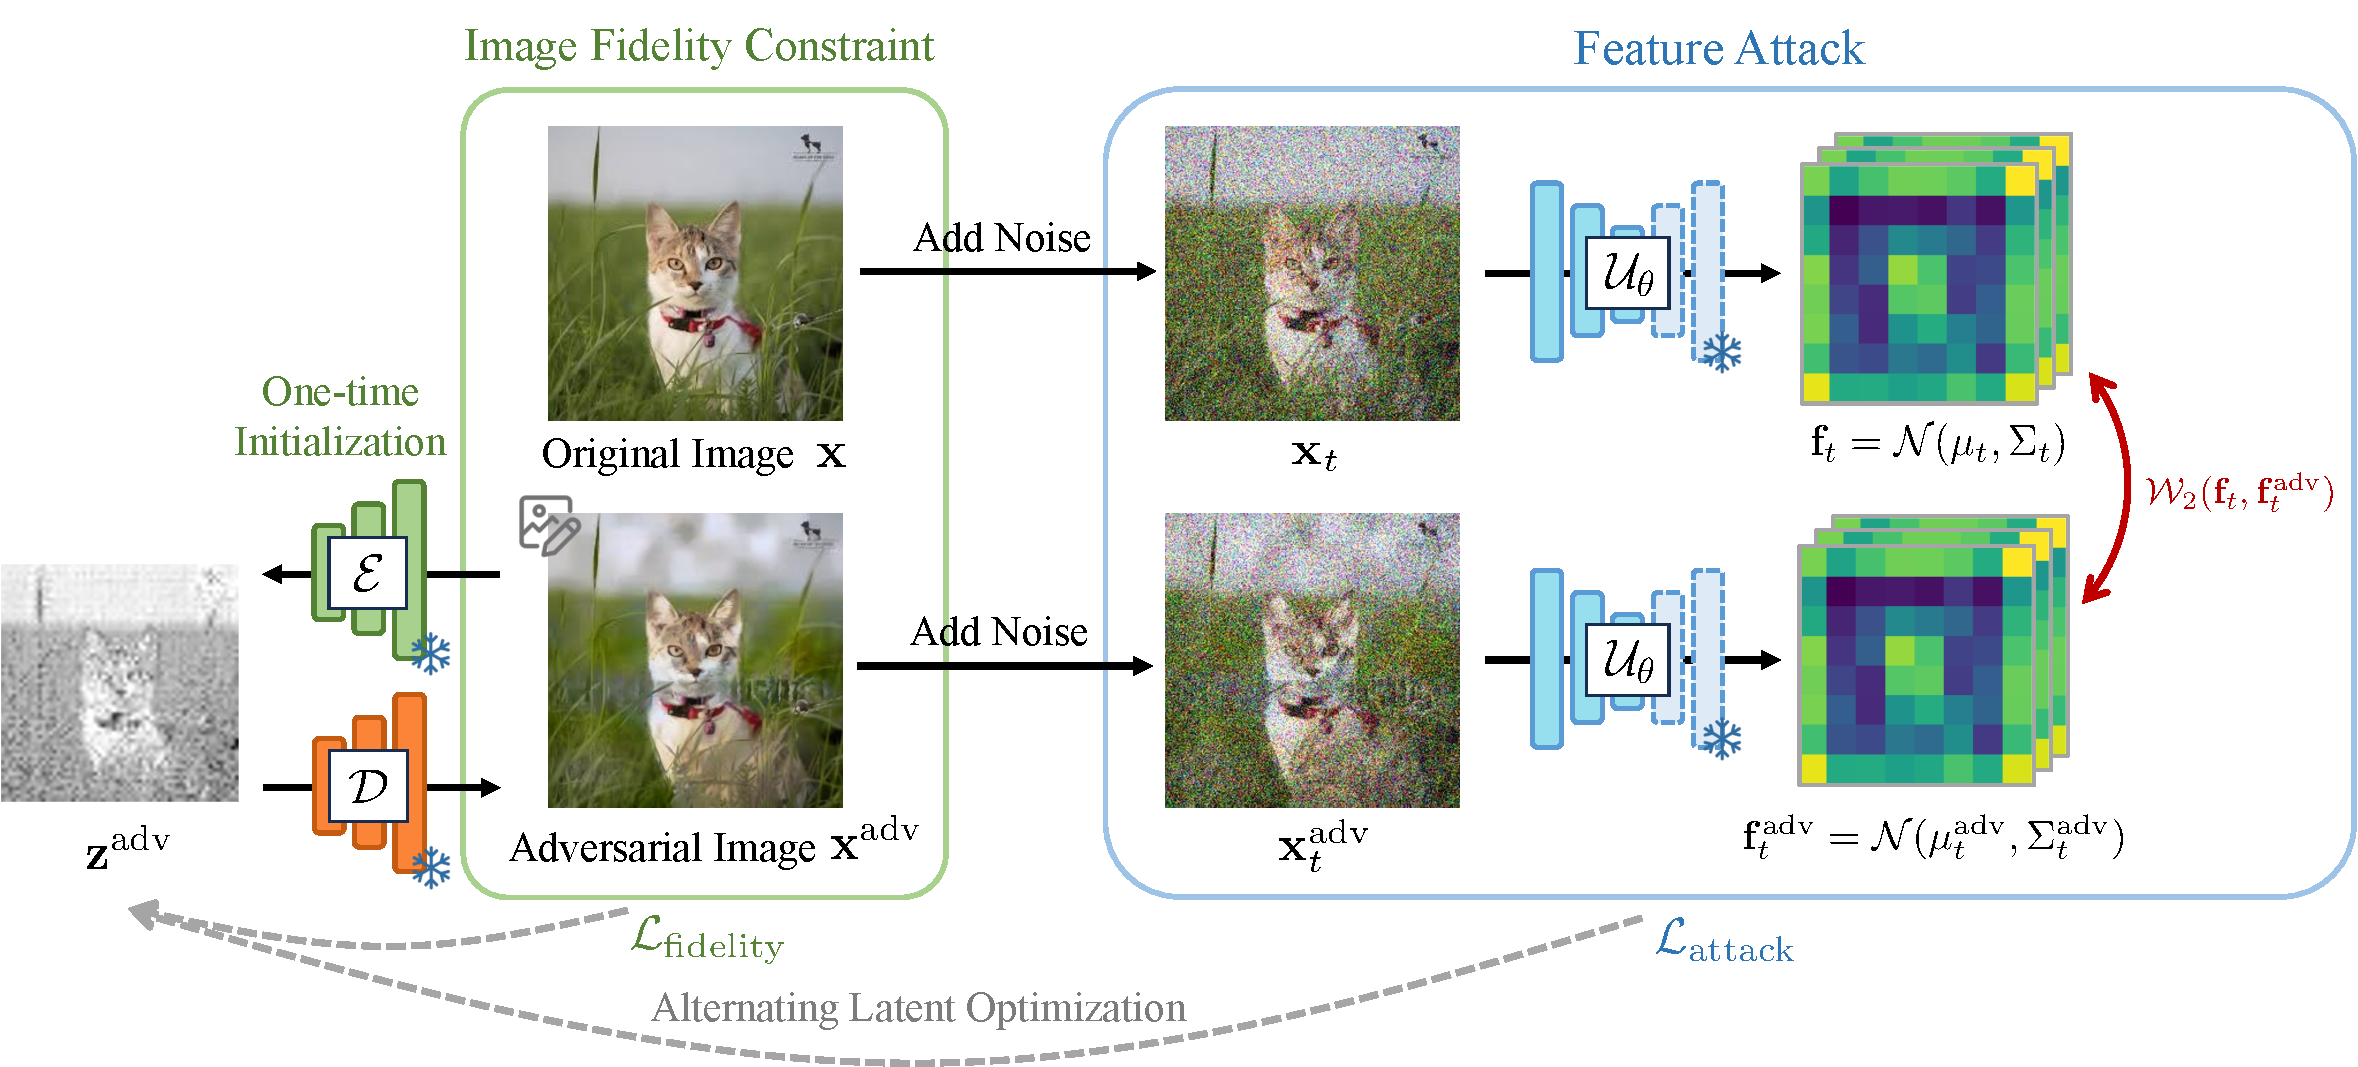
\includegraphics[width=1\linewidth]{figures/framework.pdf}
    \caption{Overview of our AtkPDM$^{+}$ algorithm: Starting from the leftmost latent of the initial adversarial image  $\mathbf{z}^{\adv}$, we first decode back to pixel-domain to perform forward diffusion with both $\mathbf{x}$ and $\mathbf{x}^{\adv}$ and feed them to frozen victim UNet. We then extract the feature representation in UNet to calculate our $\mathcal{L}_\text{attack}$, aiming to distract the recognition of image semantics. We also calculate our $\mathcal{L}_\text{fidelity}$ in pixel-domain to constrain the optimization. Finally, the $\mathbf{z}^{\adv}$ is being alternatively updated by loss gradients.}
    \label{framework}
\end{figure*}


\subsection{Overview}

To achieve effective protection against diffusion-based editing, we aim to push the protected sample away from the original clean sample by disrupting the intermediate step in the reverse diffusion process. For practical real-world applications, it's essential to ensure the protected image is perceptually similar to the original image. In practice, we uniformly sample the value of the forward diffusion step $t \sim [0, T]$ to generate noisy images and then perform optimization to craft the adversarial image $\mathbf{x}^{\adv}$ via our attacking and fidelity losses, repeating the same process $n$ times or until convergence. Figure \ref{concept} depicts these two push-and-pull criteria during different noise levels, the successful attack is reflected in the light orange line where the reverse sample moves far away from the normal edition of the image. More specifically, our method can be formulated as follows:

\begin{equation}
    \begin{aligned}
        & \max_{\mathbf{x}^{\adv} \in \mathcal{M}}
        \mathbb{E}_{
        t,
        \mathbf{x}_t| \mathbf{x}, \mathbf{x}_t^{\adv}| \mathbf{x}}
         \left[-\mathcal{L}_\text{attack}(\mathbf{x}_t, \mathbf{x}_t^{\adv})\right] \\
        & \text{subject to } \mathcal{L}_\text{fidelity}(\mathbf{x}, \mathbf{x}^{\adv}) \leq \delta,
    \end{aligned}
    \label{eq:probelm_setting_constraint}
\end{equation}

\noindent where $\delta$ denotes the attacking budget. The details of the attacking loss $\mathcal{L}_\text{attack}$ and the fidelity loss $\mathcal{L}_\text{fidelity}$ will be discussed in the following sections.


\subsubsection{Framework.}
Our framework is illustrated in Figure~\ref{framework}. We fix two identical victim UNets to extract feature representations of clean and protected samples for optimizing to push away from each other. A protection loss is jointly incorporated to constrain the optimization. After $N$ iterations, we segment out only the protecting main object of the image for better imperceptibility of image protection.

\subsection{Proposed Losses}
We propose two novel losses as optimization objectives to craft an adversarial example efficiently without running through all the diffusion steps. Attacking loss is designed to distract the feature representation in denoising UNet; Protection loss is a constraint to ensure the image quality. For notation simplicity, we first define the samples $\mathbf{x}, \mathbf{x}^{\adv}$ in different forwarded steps. 

Let $\mathcal{F}(\mathbf{x}, t, \epsilon) = \sqrt{\bar{\alpha}_t} \mathbf{x} + \sqrt{1-\bar{\alpha}_t} \epsilon$ be the diffusion forward process. Given timestep $t$ sample from $[0, T]$, noises $\epsilon_1, \epsilon_2$ sample from $\normaldist$. We denote $\mathbf{x}_t = \mathcal{F}(\mathbf{x}, t, \epsilon_1)$, and $\mathbf{x}^{\adv}_t = \mathcal{F}(\mathbf{x}^{\adv}, t, \epsilon_1)$.

\subsubsection{Attacking Loss.}
Our goal is to define effective criteria that could finally distract the reverse denoising process. PhotoGuard~\cite{salman2023raisingcostmaliciousaipowered} proposed to backpropagate through all the steps of the reverse denoising process via PGD, however, this approach is prohibitively expensive, Diff-Protect~\cite{xue2024effectiveprotectiondiffusionbased} proposed to avoid the massive cost by leveraging Score Distillation~\cite{poole2022dreamfusiontextto3dusing2d} in optimization. However, Diff-protect relies heavily on gradients of attacking encoder of an LDM as stated in their results. In PDM, we don't have such an encoder to attack; nevertheless, we find that the denoising UNet has a similar structure to encoder-decoder models, and some previous works~\cite{lin2024diffusionmodelperceptualloss, li2023fasterdiffusionrethinkingrole} characterize this property to accelerate and enhance the generation. From our observations of the feature roles in denoising UNets, we hypothesize that distracting specific inherent feature representation in UNet blocks could lead to effectively crafting an adversarial image. In practice, we first extract the feature representations of forwarded images $\mathbf{x}_t$ and $\mathbf{x}^{\adv}_t$ in frozen UNet blocks of timestep $t$. Then, we adopt 2-Wasserstein distance~\cite{arjovsky2017wasserstein} to measure the discrepancy in feature space. Note that we take the negative of the calculated distance, as we aim to pull the $\mathbf{x}^{\adv}_t$ away from $\mathbf{x}_t$. Formally, the attacking loss $\mathcal{L}_\text{attack}$ is defined as:
\begin{equation}
    \mathcal{L}_\text{attack}(\mathbf{x}_t, \mathbf{x}^{\adv}_t)
    =-\mathcal{W}_2 \left(
    \mathcal{U}^\text{(mid)}_{\theta}(\mathbf{x}_t), \mathcal{U}^\text{(mid)}_{\theta}(\mathbf{x}^{\adv}_t)
    \right).
\end{equation}

\noindent Assuming the feature distributions approximate Gaussian distributions expressed by mean $\mu_t$ and $\mu_t^{\adv}$, and non-singular covariance matrices $\Sigma_t$ and $\Sigma_t^{\adv}$. The calculation of the 2-Wasserstein distance between two normal distributions is viable through the closed-form solution~\cite{dowson1982frechet, olkin1982distance, chen2018optimal}:

\begin{equation}
    \begin{aligned}
        & \mathcal{W}_2^2(\mathcal{N}(\mu_t, \Sigma_t), \mathcal{N}(\mu_t^{\adv}, \Sigma_t^{\adv}))
        = \|\mu_t-\mu_t^{\adv}\|_2^2 \\
        & \qquad + \text{trace} (\Sigma_t + \Sigma_t^{\adv}
        -2({\Sigma_t^{\adv}}^{\frac{1}{2}}\Sigma_t{\Sigma_t^{\adv}}^{\frac{1}{2}})^\frac{1}{2} ).
    \end{aligned}
    \label{eq:wasserstein_distance}
\end{equation}

\subsubsection{Fidelity Loss.}
To control the attack budget for adversarial image quality, we design a constraint function that utilizes the feature extractor from a pretrained classifier for calculating fidelity loss. In our case, we sum up the 2-Wasserstein feature losses of $L$ different layers. Specifically, we define $\mathcal{L}_\text{fidelity}$ as:
\begin{equation}
    \mathcal{L}_\text{fidelity}(\mathbf{x}_t, \mathbf{x}^{\adv}_t)
    = \sum_{\ell=1}^L \mathcal{W}_2(\phi_\ell(\mathbf{x}), \phi_\ell(\mathbf{x}^{\adv})),
\end{equation}
where $\mathcal{W}_2$ denotes 2-Wasserstein distance and $\phi_\ell$ denotes layer $\ell$ of the feature extractor.


\subsection{Alternating Optimization for Adversarial Image}
We solve the constrained optimization problems via alternating optimization to craft the adversarial images, detailed optimization loop of AtkPDM$^{+}$ is provided in Algorithm ~\ref{alg:attdpmplus}. AtkPDM algorithm and the derivation of the alternating optimization are provided in Appendix.


\subsection{Latent Optimization via Pretrained-VAE}
Previous works suggest that diffusion models have a strong capability of resisting adversarial perturbations~\cite{xue2024pixelbarrierdiffusionmodels}, making them hard to attack via pixel-domain optimization. Moreover, they are even considered good purifiers of adversarial perturbations~\cite{nie2022diffusionmodelsadversarialpurification}. Here we propose a latent optimization strategy that crafts the ``perturbation'' in latent space. We adopt a pre-trained Variational Autoencoder (VAE) ~\cite{kingma2014autoencoding} to convert images to their latent space, and the gradients will be used to update the latent, after N iterations or losses converge, we decode back via decoder $\mathcal{D}$ to pixel domain as our final protected image. The motivation for adopting VAE is inspired by MPGD~\cite{he2024manifold}. This strategy is effective for crafting a robust adversarial image against pixel-domain diffusion models while also better preserving the protection quality rather than only incorporating fidelity constraints. The constraint optimization thereby becomes: 
\begin{equation}
\begin{aligned}
    & \max_{\mathbf{z}^{\adv}}
    \mathbb{E}_{
    t,
    \mathbf{x}_t| \mathbf{x}, \mathbf{x}_t^{\adv}| \mathcal{D}(\mathbf{z}^{\adv})}
    \left[-\mathcal{L}_\text{attack}(\mathbf{x}_t, \mathbf{x}_t^{\adv})\right] \\
    & \text{subject to } \mathcal{L}_\text{fidelity}(\mathbf{x}, \mathcal{D}(\mathbf{z}^{\adv})) \leq \delta.
\end{aligned}
\label{eq:probelm_setting_constraint}
\end{equation}

\noindent Detailed latent optimization loop is provided in Algorithm~\ref{alg:attdpmplus}.


\begin{algorithm}[t]
    \caption{AtkPDM$^{+}$}
    \label{alg:attdpmplus}
    \small{
    \begin{algorithmic}[1] 
        \STATE{\textbf{Input:}
        Image to be protected $\mathbf{x}$, attack budget $\delta > 0$, step size $\gamma_1, \gamma_2>0$, \textcolor{black}{VAE encoder $\mathcal{E}$, and VAE decoder $\mathcal{D}$}}
        \STATE{\textbf{Initialization:} $\mathbf{x}^{\adv} \leftarrow \mathbf{x}$, $L_\text{attack} \leftarrow \infty$}
        \STATE{\textcolor{black}{Encode adversarial image to latent space: $\mathbf{z}^{\adv} \leftarrow \mathcal{E}(\mathbf{x}^{\adv})$}}
        \WHILE{$L_\text{attack}$ not convergent}
            \STATE{\textcolor{black}{Decode adversarial latent to pixel space: $\mathbf{x}^{\adv} \leftarrow \mathcal{D}(\mathbf{z}^{\adv})$}}
            \STATE{Sample timestep: $t \sim [0, T]$}
            \STATE{Sample noise: $\epsilon_1, \epsilon_2 \sim \normaldist$}
            \STATE{Compute original noisy sample: $\mathbf{x}_t \leftarrow \mathcal{F}(\mathbf{x}, t, \epsilon_1)$}
            \STATE{Compute adversarial noisy sample: $\mathbf{x}^{\adv}_t \leftarrow \mathcal{F}(\mathbf{x}^{\adv}, t, \epsilon_2)$}
            \STATE{\textcolor{black}{Update $\mathbf{z}^{\adv}$ by Gradient Descent: \\
            $\mathbf{z}^{\adv} \leftarrow \mathbf{z}^{\adv} -
            \gamma_1 \sign(\nabla_{\mathbf{z}^{\adv}} \mathcal{L}_\text{attack}(\mathbf{x}_t, \mathbf{x}^{\adv}_t))$}}
            \WHILE{$\mathcal{L}_\text{fidelity}(\mathbf{x}, \textcolor{black}{\mathcal{D}(\mathbf{z}^{\adv})}) > \delta$}
            \STATE{ 
            \textcolor{black}{$\mathbf{z}^{\adv} \leftarrow \mathbf{z}^{\adv} -
            \gamma_2 \nabla_{\mathbf{z}^{\adv}} \mathcal{L}_\text{fidelity}(\mathbf{x}, \mathcal{D}(\mathbf{z}^{\adv}))$}}
            \ENDWHILE
        \ENDWHILE
        \STATE{\textcolor{black}{Decode adversarial latent to pixel space: $\mathbf{x}^{\adv} \leftarrow \mathcal{D}(\mathbf{z}^{\adv})$}}
        \RETURN {$\mathbf{x}^{\adv}$}
    \end{algorithmic}
    }
\end{algorithm}


\section{Experiment Results}
In this section, we examine the attack effectiveness and robustness of our approach under extensive settings. 


\begin{table}[tb]
    \centering
    \setlength{\tabcolsep}{1mm}
    \vspace{-2ex}
    \resizebox{1\columnwidth}{!}{
    \begin{tabular}{l|ccc|ccc}
    \toprule
        \multirow{2}{*}{Methods} &  \multicolumn{3}{@{}c}{{\bf GSM8K}} &  \multicolumn{3}{@{}c}{{\bf BBH}} \\
         & EM & Tokens & $1/\tau$ & EM & Tokens & $1/\tau$\\
        % \hline
         \cmidrule (r){1-1}\cmidrule (lr){2-4} \cmidrule (lr){5-7}
     Full-shot & 78.85 & 2,366 & - & 70.07 & 774 & -  \\
     \hline
     \hline
     \multicolumn{4}{@{}l}{{\bf \textit{1-shot constraint}}} \\ 
    1-shot & 77.10 & 422 & 6x & 69.60 & 284 & 3x \\
    Selective-Context & 53.98 & 452 & 5x & 54.27 & 276 & 3x \\
    GPT4 Generation & 71.87 & 496 & 5x & 27.13 & 260 & 3x \\
    {\cellcolor[rgb]{0.925,0.957,1}}\textbf{Ours} & {\cellcolor[rgb]{0.925,0.957,1}}\textbf{79.08} & {\cellcolor[rgb]{0.925,0.957,1}}446 & {\cellcolor[rgb]{0.925,0.957,1}}5x & {\cellcolor[rgb]{0.925,0.957,1}}\textbf{70.11} & {\cellcolor[rgb]{0.925,0.957,1}}288 & {\cellcolor[rgb]{0.925,0.957,1}}3x \\
     \hline
     \hline
     \multicolumn{4}{@{}l}{{\bf \textit{half-shot constraint}}} \\ 
    Sentence Selection & 72.33 & 230 & 10x & 39.56 & 175 & 4x\\
    Selective-Context & 52.99 & 218 & 11x & 54.02 & 155 & 5x \\
    GPT4 Generation & 68.61 & 223 & 11x & 27.09 & 161 & 5x \\
    {\cellcolor[rgb]{0.925,0.957,1}}\textbf{Ours} & {\cellcolor[rgb]{0.925,0.957,1}}\textbf{77.41} & {\cellcolor[rgb]{0.925,0.957,1}}171 & {\cellcolor[rgb]{0.925,0.957,1}}14x & {\cellcolor[rgb]{0.925,0.957,1}}\textbf{61.60} & {\cellcolor[rgb]{0.925,0.957,1}}171 & {\cellcolor[rgb]{0.925,0.957,1}}5x \\
     \hline
     \hline
     \multicolumn{4}{@{}l}{{\bf \textit{quarter-shot constraint}}} \\ 
    Sentence Selection & 66.67 & 195 & 12x & 46.00 & 109 & 7x \\
    Selective-Context & 44.20 & 157 & 15x & 47.37 & 108 & 7x \\
    GPT4 Generation & 56.33 & 188 & 20x & 26.81 & 101 & 8x \\
    {\cellcolor[rgb]{0.925,0.957,1}}\textbf{Ours} & {\cellcolor[rgb]{0.925,0.957,1}}\textbf{77.33} & {\cellcolor[rgb]{0.925,0.957,1}}117 & {\cellcolor[rgb]{0.925,0.957,1}}20x & {\cellcolor[rgb]{0.925,0.957,1}}\textbf{56.85} & {\cellcolor[rgb]{0.925,0.957,1}}110 & {\cellcolor[rgb]{0.925,0.957,1}}7x \\
     \hline
     \hline
    zero-shot & 48.75$^{\dag}$ & 11 & 215x & 32.32 & 16 & 48x \\
    Simple Prompt & 74.9 & 691 & 3x & - & - & - \\
    \bottomrule
    \end{tabular}
    }
    \caption{Performance of different methods under different target compression ratios on the GSM8K mathematical reasoning and Big-bench Hard (BBH) datasets. $^{\dag}$We also include the instruction of the prompt in zero-shot experiments for a vertical comparison.}
    \label{tab:main_results}
\end{table}



\begin{table}[t]
\footnotesize{
    \centering
    \begin{tabular}{lcccc}
        \toprule
        \multirow{2}{*}{Defense Method} & \multicolumn{4}{c}{Attacking Effectiveness} \\ 
         &  SSIM $\downarrow$ & PSNR $\downarrow$ & LPIPS $\uparrow$ & IA-Score $\downarrow$ \\
        \midrule
        Crop-and-Resize & 0.68 & 29.28 & 0.42 & 0.79 \\
        JPEG Comp. & 0.78  & 29.82 & 0.36 & 0.79 \\
        \midrule
        None & 0.79 & 30.05 & 0.33 & 0.81 \\
        \bottomrule
    \end{tabular}
    \caption{Quantitative results of our adversarial images against defense methods. Both Crop-and-Resize and JPEG Compression fail to defend our attack. ``None'' indicates no defense is applied, as the baseline for comparison.}
    % The term "None" in the defense method column indicates the use of the adversarial image generated by our method without applying any purification techniques.
\label{tab:defense}
}
\end{table}



\subsection{Experiment Settings}
\subsubsection{Implementation Details.} We conduct all our experiments in white box settings and examine the effectiveness of our attacks using SDEdit \cite{meng2021sdedit}. For the Variational Autoencoder (VAE) ~\cite{kingma2014autoencoding} in our AtkPDM$^{+}$, we utilize the VAE provided by StableDiffusion V1.5 ~\cite{rombach2022high}.
We run all of our experiments with 300 optimization steps, which is empirically determined, to balance attacking effectiveness and image protection quality with reasonable speed. Other loss parameters and running time are provided in the Appendix. The implementation is built on the Diffusers library. All the experiments are conducted with a single Nvidia Tesla V100 GPU.


\subsubsection{Victim Models and Datasets.}
We test our approach on PDMs with three open-source checkpoints on HuggingFace, specifically ``google/ddpm-ema-church-256'', ''google/ddpm-cat-256'' and ``google/ddpm-ema-celebahq-256''. For the results reported in Table~\ref{tab:attackPDM}, we run 30 images for each victim model. Additionally, for generalizability in practical scenarios, we synthesize the data with half randomly from the originally trained dataset and another half from randomly crawled with keywords from the Internet.

\subsubsection{Baseline Methods and Evaluation Metrics.}

To the best of our knowledge, previous methods have mainly focused on LDMs, and effective PDM attacks have not yet been developed, however, we still implement Projected Gradient Ascent (PGAscent) with their proposed semantic loss by~\cite{salman2023raisingcostmaliciousaipowered, liang2023adversarialexampledoesgood, liang2023mistimprovedadversarialexamples, xue2024effectiveprotectiondiffusionbased}. Notably, Diff-Protect~\cite{xue2024effectiveprotectiondiffusionbased} proposed to minimize the semantic loss is surprisingly better than maximizing the semantic loss, we also adopted this method in attacking PDMs and denote as Diff-Protect. To quantify the adversarial image visual quality, we adopted Structural Similarity (SSIM) ~\cite{wang2004image}, Peak Signal-to-Noise Ratio (PSNR), and Learned Perceptual Image Patch Similarity (LPIPS) ~\cite{zhang2018unreasonable}. We also inherit these three metrics, but negatively to quantify the effectiveness of our attack. We also adopted Image Alignment Score (IA-Score) \cite{kumari2023multi} that leverages CLIP \cite{radford2021learning} to calculate the cosine similarity of image encoder features. In distinguishing from previous methods, to more faithfully reflect the attack effectiveness, we fix the same seed of the random generator when generating clean and adversarial samples, then calculate the scores based on the paired samples.

\subsection{Attack Effectiveness on PDMs}

As quantitatively reported in Table~\ref{tab:attackPDM} and qualitative results in Figure~\ref{qualitative}, compared to previous PGD-based methods incorporating semantic loss, i.e., negative training loss of diffusion models, our method exhibits superior performance in both adversarial image quality and attacking effectiveness. And our reported figures has generally stable as reflected in lower standard deviation. It is worth noting that even if the adversarial image qualities of the PGD-based methods are far worse than ours, their attacking effectiveness still falls short, suggesting that PDMs are robust against traditional perturbation methods, this finding is also aligned with previous works~\cite{xue2024effectiveprotectiondiffusionbased,xue2024pixelbarrierdiffusionmodels}. For AtkPDM$^+$, combined with our latent optimization strategy, the adversarial image quality has enhanced while slightly affecting the attacking effectiveness, still outperforming the previous methods.



\begin{table}[t]
\footnotesize{
    \centering
    \begin{tabular}{lcccc}
        \toprule
        \multirow{2}{*}{Setting} & \multicolumn{4}{c}{Attacking Effectiveness} \\ 
         &  SSIM $\downarrow$ & PSNR $\downarrow$ & LPIPS $\uparrow$ & IA-Score $\downarrow$ \\
        \midrule
        White Box & 0.79 & 30.05 & 0.33 & 0.81 \\
        
        Black Box & 0.86 & 30.25 & 0.29 & 0.85 \\
    
        \midrule
        Difference & 0.07 & 0.20 & 0.04 & 0.04 \\
        \bottomrule
    \end{tabular}
    \caption{Quantitative results of black box attack. We use the same set of adversarial images and feed to white box and black box models to examine the black box transferability.} 
\label{tab:blackBox}
}
\end{table}
\begin{figure*}[t]
\centering
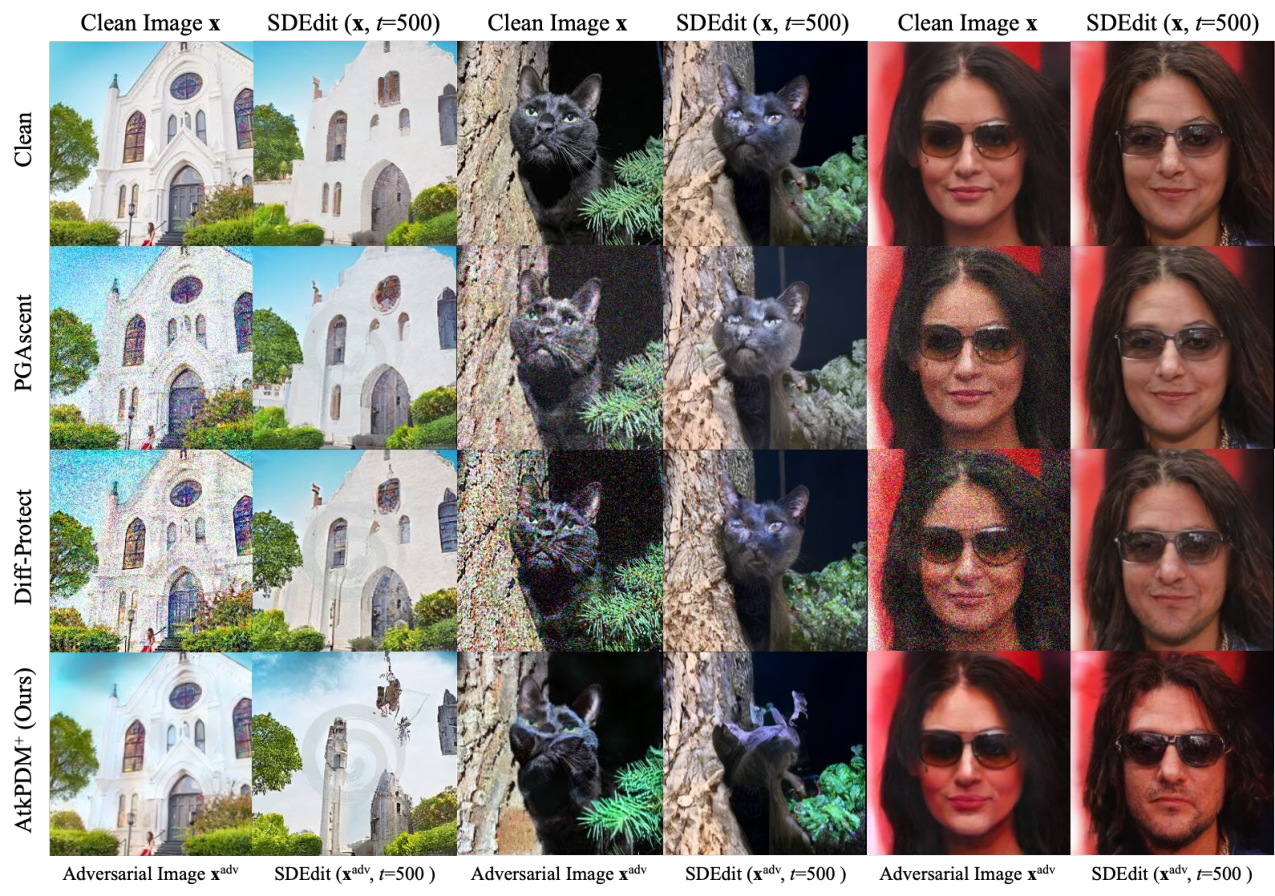
\includegraphics[width=0.79\linewidth]{figures/qualitative_results.pdf}
\caption{Qualitative results compared to previous methods: our adversarial images can effectively corrupt the edited results without significant fidelity decrease. The same column shares the same random seed for fair comparison.
}
\label{qualitative}
\end{figure*}

\begin{table*}
    \centering
    \small{
    \begin{tabular}{lc|ccc|cccc}
        \toprule
        \multirow{2}{*}{Losses} & \multirow{2}{*}{VAE} & \multicolumn{3}{c|}{Adversarial Image Quality} & \multicolumn{4}{c}{Attacking Effectiveness} \\ 
         & & SSIM $\uparrow$ & PSNR $\uparrow$ & LPIPS $\downarrow$ & SSIM $\downarrow$ & PSNR $\downarrow$ & LPIPS $\uparrow$ & IA-Score $\downarrow$ \\
        \midrule
        $\mathcal{L}_\text{semantic}$ &  & 0.37 $\pm$ 0.09  & 28.17 $\pm$ 0.22 & 0.73 $\pm$ 0.16  & 0.89 $\pm$ 0.05 & 31.06 $\pm$ 1.94 & 0.17 $\pm$ 0.09 & 0.93 $\pm$ 0.04 \\
        $\mathcal{L}_\text{semantic}$ & \checkmark & 0.80 $\pm$ 0.05 & \second{29.78} $\pm$ 0.42 & \second{0.17} $\pm$ 0.03 & 0.82 $\pm$ 0.05 & 30.43 $\pm$ 0.75 & 0.15 $\pm$ 0.06 & 0.92 $\pm$ 0.04 \\
        % $\mathcal{L}_\text{semantic}$ + $\mathcal{L}_\text{fidelity}$ &  & 0.12  & 27.90 & 1.08 & \first{0.58} & \first{28.01} & \first{0.93} & \first{0.61} \\ 
        $\mathcal{L}_\text{semantic}$ + $\mathcal{L}_\text{fidelity}$ & \checkmark & \first{0.82} $\pm$ 0.05 & \first{30.30} $\pm$ 0.81 & \first{0.13} $\pm$ 0.03 & 0.90 $\pm$ 0.03 & 31.24 $\pm$ 1.19 & 0.08 $\pm$ 0.03 & 0.96 $\pm$ 0.02 \\
        \midrule
        $\mathcal{L}_\text{attack}$ + $\mathcal{L}_\text{fidelity}$ (Ours) & & 0.75 $\pm$ 0.03 & 28.22 $\pm$ 0.10  & 0.26 $\pm$ 0.04 & \first{0.75} $\pm$ 0.04 & \first{29.61} $\pm$ 0.23 & \first{0.40} $\pm$ 0.05 & \first{0.76} $\pm$ 0.06 \\
        $\mathcal{L}_\text{attack}$ + $\mathcal{L}_\text{fidelity}$ (Ours) & \checkmark & \second{0.81} $\pm$ 0.03 & 28.64 $\pm$ 0.19 & \first{0.13} $\pm$ 0.02 & \second{0.79} $\pm$ 0.04 & \second{30.05} $\pm$ 0.47 & \second{0.33} $\pm$ 0.07 & \second{0.81} $\pm$ 0.06 \\
        \bottomrule
    \end{tabular}
    }
    \caption{Quantitative results of ablation study. The best is in bold and the second best is underlined. Errors denote one standard deviation of all images in our test datasets.}
    \label{tab:loss_ablation}
    \vspace*{-10pt}
\end{table*}



\subsection{Against Defense Methods}
We examine the robustness of our approach against two widely recognized and effective defense methods for defending against adversarial attacks as reported in Table~\ref{tab:defense}.

\subsubsection{Crop and Resize.}
Noted by Diff-Protect, crop and resize is simple yet the most effective defense method against their attacks on LDMs. We also test our method against this defense using their settings, i.e., cropping 20\% of the adversarial image and then resizing it to its original dimensions.


\subsubsection{JPEG Compression.}
Sandoval-Segura et al.~\cite{sandoval2023jpeg} demonstrated that JPEG compression is a simple yet effective adversarial defense method. In our experiments, we implement the JPEG compression at a quality setting of 25\%. The quantitative results in Table~\ref{tab:defense} demonstrate that our method is robust against these two defense methods, with four of the metrics listed in Table~\ref{tab:defense} are not worse than no defenses. Surprisingly, these defense methods even make the adversarial image more effective than cases without defense.


\subsection{Black Box Transferability}
We craft adversarial images with the proxy model, ``google/ddpm-ema-church-256'', in white-box settings and test their transferability to another ``google/ddpm-bedroom-256'' model for black-box attacks. Under identical validation settings, Table~\ref{tab:blackBox} reveals only a slight decrease in attack effectiveness metrics, indicating successful black-box transferability.



\subsection{Effectiveness of Latent Optimization via VAE}
We first incorporate our VAE latent optimization strategy in the previous semantic-loss-based PGAscent. From Table~\ref{tab:loss_ablation}, without using $\mathcal{L}_\text{fidelity}$, latent optimization has significantly enhanced the adversarial image quality and even slightly improved the attacking effectiveness. Adopting latent optimization in our approach enhances visual quality with a negligible decrease in attacking effectiveness. Surprisingly, incorporating our $\mathcal{L}_\text{fidelity}$ with current PGD-based method will drastically decrease the adversarial image quality despite its attack performing better than ours. This may be due to different constrained optimization problem settings.

\section{Discussion}
% \subsection{Concurrent Work}
% In recent years it has become more popular to release ``uncensored'' language models, and with that there have been tools and techniques developed to detect undesirable outputs produced by these models. One such tool is Llama Guard \cite{inan2023llama}, a large language model designed to perform both prompt- and response-classification to maximise the safety of chat systems. Like DPH, Llama Guard can be used to detect and reject harmful outputs produced by a language model. However, unlike DPH, Llama Guard is an entirely separate model which must be run concurrently with chat model and therefor increases the compute and memory requirements of the combined system. % this especially contrasts with DPH being especially suited for small language models which inherently require a much smaller compute budget.

\subsection{Future Work}
As shown in the results section, DPH is capable of learning to assign higher rewards to preferred outputs and lower rewards to dispreferred outputs which implies the pooling function learns rich features with respect to prompt-completion pairs. We believe that it would be possible to also extract additional information from the output of the pooling function to detect finer grained signals such as helpfulness, humor, creativity, toxic content, etc. This can be achieved by training on a conversational dataset such Open Assistant \cite{köpf2023openassistant} which contains a variety of human-curated labels in addition to machine-generated labels produced by Detoxify \cite{Detoxify}.

% It is also worth examining how the performance of DPH scales with larger language models, and if it can be used as a post-hoc technique to provide safety guardrails for uncensored language models such as Mistral 7B and observe how it performs compared to systems such as Llama Guard while maintaining much lower compute requirements.

\subsection{Limitations}
The main benefit of DPH being its ability to perform alignment without directly effecting the model's output distribution is also its main limitation: unlike other alignment techniques which can help prevent the model generating harmful outputs, DPH is only capable of \textit{detecting} harmful outputs. Although we do include DPO alignment in our experiments to reduce the likelihood of harmful outputs, DPH does not require such model alignment to function, which shifts the responsibility of rejecting harmful outputs to the end user or service provider.

\subsection{Conclusion}
In this paper we introduced Direct Preference Heads, a novel form of language model alignment which is performed at inference time to prune candidate completions for a given prompt. Unlike other alignment techniques which coerce the model into generating human preference aligned outputs, DPH instead produces reward scores for candidate outputs without affecting the actual generation process and therefor avoids the issue of RLHF leading to degraded performance when applied to smaller language models. We formulated two loss functions for DPH and find strong connections to Conservative DPO, implying that DPH is robust to label noise and can be tuned to a specific confidence margin. Finally, we evaluated our methods on a number of NLU, commonsense reasoning and reading Comprehension tasks and found that DPH is able to consistently outperform both our SFT baseline and multiple publicly available language model checkpoints of varying size and training volume.

\subsection*{Broader Impacts}
As with all language modeling systems we cannot guarantee all responses produced by our models are factually correct nor can we guarantee that they are safe and free from harmful content. Our work focuses on creating a system that helps filter out incorrect and harmful messages by scoring candidate outputs, but as with all alignment techniques our models may be susceptible to so-called `jailbreaks' which can coerce the model into incorrectly assigning a higher score to less desirable content. To maximise safety DPH should be implemented alongside other safety guardrails such as Llama Guard \cite{inan2023llama} when used for publicly facing chat systems, and we intend for our provided model checkpoints to be used for reproduction of results and further research in the field of alignment.

\bibliography{main}

% \clearpage
\section*{AAAI Checklist}
\subsection*{Conceptual and Methodological Details}
\begin{itemize}
    \item[] Includes a conceptual outline and/or pseudocode description of AI methods introduced: \textbf{yes}
    \item[] Clearly delineates statements that are opinions, hypothesis, and speculation from objective facts and results: \textbf{yes}
    \item[] Provides well marked pedagogical references for less-familiar readers to gain background necessary to replicate the paper: \textbf{yes}
\end{itemize}

\subsection*{Theoretical Contributions}
Does this paper make theoretical contributions? \textbf{no}

If yes, please complete the list below:
\begin{itemize}
    \item[] All assumptions and restrictions are stated clearly and formally: \textbf{(yes/partial/no)}
    \item[] All novel claims are stated formally (e.g., in theorem statements): \textbf{(yes/partial/no)}
    \item[] Proofs of all novel claims are included: \textbf{(yes/partial/no)}
    \item[] Proof sketches or intuitions are given for complex and/or novel results: \textbf{(yes/partial/no)}
    \item[] Appropriate citations to theoretical tools used are given: \textbf{(yes/partial/no)}
    \item[] All theoretical claims are demonstrated empirically to hold: \textbf{(yes/partial/no/NA)}
    \item[] All experimental code used to eliminate or disprove claims is included: \textbf{(yes/no/NA)}
\end{itemize}

\subsection*{Dataset Usage}
Does this paper rely on one or more datasets? \textbf{yes}

If yes, please complete the list below:
\begin{itemize}
    \item[] A motivation is given for why the experiments are conducted on the selected datasets: \textbf{yes}
    \item[] All novel datasets introduced in this paper are included in a data appendix: \textbf{NA}
    \item[] All novel datasets introduced in this paper will be made publicly available upon publication of the paper with a license that allows free usage for research purposes: \textbf{NA}
    \item[] All datasets drawn from the existing literature (potentially including authors' own previously published work) are accompanied by appropriate citations: \textbf{yes}
    \item[] All datasets drawn from the existing literature (potentially including authors' own previously published work) are publicly available: \textbf{yes}
    \item[] All datasets that are not publicly available are described in detail, with explanation why publicly available alternatives are not scientifically satisficing: \textbf{NA}
\end{itemize}

\subsection*{Computational Experiments}
Does this paper include computational experiments? \textbf{yes}

If yes, please complete the list below:
\begin{itemize}
    \item[] Any code required for pre-processing data is included in the appendix: \textbf{no}
    \item[] All source code required for conducting and analyzing the experiments is included in a code appendix: \textbf{no}
    \item[] All source code required for conducting and analyzing the experiments will be made publicly available upon publication of the paper with a license that allows free usage for research purposes: \textbf{yes}
    \item[] All source code implementing new methods have comments detailing the implementation, with references to the paper where each step comes from: \textbf{yes}
    \item[] If an algorithm depends on randomness, then the method used for setting seeds is described in a way sufficient to allow replication of results: \textbf{partial}
    \item[] This paper specifies the computing infrastructure used for running experiments (hardware and software), including GPU/CPU models; amount of memory; operating system; names and versions of relevant software libraries and frameworks: \textbf{partial}
    \item[] This paper formally describes evaluation metrics used and explains the motivation for choosing these metrics: \textbf{yes}
    \item[] This paper states the number of algorithm runs used to compute each reported result: \textbf{partial}
    \item[] Analysis of experiments goes beyond single-dimensional summaries of performance (e.g., average; median) to include measures of variation, confidence, or other distributional information: \textbf{yes}
    \item[] The significance of any improvement or decrease in performance is judged using appropriate statistical tests (e.g., Wilcoxon signed-rank): \textbf{no}
    \item[] This paper lists all final (hyper-)parameters used for each model/algorithm in the paper's experiments: \textbf{yes}
    \item[] This paper states the number and range of values tried per (hyper-) parameter during development of the paper, along with the criterion used for selecting the final parameter setting: \textbf{partial}
\end{itemize}

\clearpage
\appendix

\begin{center}
    \LARGE{\textbf{Supplementary Material}}
\end{center}

\section{More Implementation Details}
The feature extractor for calculating $\mathcal{L}_\text{fidelity}$ is VGG16~\cite{Simonyan2014VeryDC} with IMAGENET1K-V1 checkpoint. We use the SDEdit with the forward step $t=500$ for our main study results as it balances faithfulness to the original image and flexibility for editing. Empirically, we choose to randomly sample the forward step $t \sim [0, 500]$ to enhance the optimization efficiency. The average time to optimize 300 steps for an image on a single Nvidia Tesla V100 is about 300 seconds. The estimated average memory usage is about 24GB. Table \ref{tab:step_size} provides the details of the step sizes that we use to attack different models. 

\begin{table}[h]
\footnotesize{
    \centering
    \begin{tabular}{lccc}
        \toprule
        \multirow{2}{*}{Models} & \multicolumn{2}{c}{Step Size} \\ 
         &  $\gamma_1$ ($\mathcal{L}_\text{attack}$)  & $\gamma_2$ ($\mathcal{L}_\text{fidelity}$)   \\
        \midrule
        google/ddpm-ema-church-256 & $100/255$ & $40/255$ \\
        google/ddpm-cat-256 & $100/255$ & $5/255$ \\
        google/ddpm-ema-celebahq-256 & $50/255$ & $35/255$ \\  
        
        \bottomrule
    \end{tabular}
    \caption{The step sizes used for different models during optimization.} 
\label{tab:step_size}
}
\end{table}


\section{More Experimental Results}

\subsection{Attack Effectiveness on Latent Diffusion Models}
We propose the feature representation attacking loss which can be adapted to target any UNet-based diffusion models. Hence, it is applicable to attack LDM using our proposed framework. We follow the evaluation settings of the previous works~\cite{xue2024effectiveprotectiondiffusionbased} for fair comparisons. Quantitative results are shown in Table~\ref{tab:attackLDM}. Compared to previous LDM-specified methods, our method could achieve comparable results. This finding reflects the general vulnerability in UNet-based diffusion models that can be exploited to craft adversarial images against either PDMs or LDMs. 

\begin{table*}[t]
    \centering
    \small{
    \begin{tabular}{ll|ccc|cccc}
        \toprule
        & \multirow{2}{*}{Methods} & \multicolumn{3}{c|}{Adversarial Image Quality} & \multicolumn{4}{c}{Attacking Effectiveness} \\ 
         & & SSIM $\uparrow$ & PSNR $\uparrow$ & LPIPS $\downarrow$ & SSIM $\downarrow$ & PSNR $\downarrow$ & LPIPS $\uparrow$ & IA-Score $\downarrow$ \\
        \midrule
        \multirow{6}{*}{\rotatebox{90}{Church}}
        & AdvDM ($+$) & \first{0.85} $\pm$ 0.03 & \first{30.42} $\pm$ 0.15 & \second{0.23} $\pm$ 0.06 & 0.19 $\pm$ 0.05 & 28.00 $\pm$ 0.16 & 0.71 $\pm$ 0.04 & 0.49 $\pm$ 0.06 \\
        & Mist ($+$) & 0.81 $\pm$  0.03 & 29.45 $\pm$ 0.13 & 0.25 $\pm$ 0.05 & \first{0.14} $\pm$ 0.03 & \first{27.95} $\pm$ 0.13 & \first{0.76} $\pm$ 0.04 & \second{0.48} $\pm$ 0.05 \\
        & Diff-Protect ($-$) & 0.79 $\pm$ 0.03 & 29.92 $\pm$ 0.15 & 0.24 $\pm$ 0.06 & \second{0.15} $\pm$ 0.03 & 28.00 $\pm$ 0.14 & 0.71 $\pm$ 0.04 & \second{0.48} $\pm$ 0.05 \\
        & Diff-Protect ($+$) & 0.79 $\pm$ 0.04 & 29.47 $\pm$ 0.11 & 0.26 $\pm$ 0.06 & 0.17 $\pm$ 0.04 & 28.00 $\pm$ 0.15 & 0.69 $\pm$ 0.04 & 0.49 $\pm$ 0.06 \\
        & AtkPDM (Ours) & \second{0.82} $\pm$ 0.02 & \second{30.40} $\pm$ 0.27 & 0.24 $\pm$ 0.05 & \first{0.14} $\pm$ 0.03 & \second{27.96} $\pm$ 0.17 & \second{0.74} $\pm$ 0.02 & \first{0.47} $\pm$ 0.04  \\
        & AtkPDM$^+$ (Ours) & 0.61 $\pm$ 0.07 & 29.17 $\pm$ 0.32 & \first{0.20} $\pm$ 0.02 & 0.27 $\pm$ 0.06 & 28.07 $\pm$ 0.18 & 0.66 $\pm$ 0.05 & 0.51 $\pm$ 0.06 \\
        \midrule
        \multirow{6}{*}{\rotatebox{90}{Cat}}
        & AdvDM ($+$) & \first{0.86} $\pm$ 0.04 & \second{30.68} $\pm$ 0.24 & \second{0.25} $\pm$ 0.09 & 0.21 $\pm$ 0.05 & 28.03 $\pm$ 0.21 & 0.70 $\pm$ 0.07 & \second{0.53} $\pm$ 0.04 \\
        & Mist ($+$) & 0.81 $\pm$ 0.04 & 29.63 $\pm$ 0.22 & 0.27 $\pm$ 0.08 & \first{0.14} $\pm$ 0.04 & \first{27.96} $\pm$ 0.17 & \first{0.77} $\pm$ 0.06 & \first{0.52} $\pm$ 0.04 \\
        & Diff-Protect ($-$) & 0.78 $\pm$ 0.05 & 30.12 $\pm$ 0.24 & 0.27 $\pm$ 0.08 & \second{0.16} $\pm$ 0.05 & \first{27.96} $\pm$ 0.15 & \second{0.72} $\pm$ 0.06 & \first{0.52} $\pm$ 0.03 \\
        & Diff-Protect ($+$) & 0.77 $\pm$ 0.06 & 29.56 $\pm$ 0.16 & 0.28 $\pm$ 0.09 & 0.17 $\pm$ 0.05 & \second{27.98} $\pm$ 0.16 & 0.71 $\pm$ 0.06 & \second{0.53} $\pm$ 0.04 \\
        & AtkPDM (Ours) & \second{0.84} $\pm$ 0.02 & \first{30.79} $\pm$ 0.49 & \second{0.25} $\pm$ 0.07 & 0.18 $\pm$ 0.04 & 28.00 $\pm$ 0.19 & \second{0.72} $\pm$ 0.05 & \first{0.52} $\pm$ 0.03  \\
        & AtkPDM$^+$ (Ours) & 0.68 $\pm$ 0.13 & 29.68 $\pm$ 0.74 & \first{0.16} $\pm$ 0.03 & 0.31 $\pm$ 0.10 & 28.13 $\pm$ 0.27 & 0.64 $\pm$ 0.06 & 0.54 $\pm$ 0.04 \\
        \midrule
        \multirow{6}{*}{\rotatebox{90}{Face}}
        & AdvDM ($+$) & \first{0.83} $\pm$ 0.02 & \second{30.81} $\pm$ 0.22 & 0.32 $\pm$ 0.06 & 0.26 $\pm$ 0.05 & 28.07 $\pm$ 0.28 & 0.74 $\pm$ 0.05 & 0.47 $\pm$ 0.07 \\
        & Mist ($+$) & 0.79 $\pm$ 0.03 & 29.75 $\pm$ 0.22 & 0.34 $\pm$ 0.06 & \first{0.19} $\pm$ 0.05 & \first{27.99} $\pm$ 0.21 & \first{0.81} $\pm$ 0.05 & 0.46 $\pm$ 0.08 \\
        & Diff-Protect ($-$) & 0.74 $\pm$ 0.04 & 30.34 $\pm$ 0.13 & 0.33 $\pm$ 0.06 & \second{0.21} $\pm$ 0.05 & \second{28.03} $\pm$ 0.21 & 0.76 $\pm$ 0.06 & \second{0.45} $\pm$ 0.07 \\
        & Diff-Protect ($+$) & 0.72 $\pm$ 0.05 & 29.68 $\pm$ 0.09 & 0.36 $\pm$ 0.06 & \second{0.21} $\pm$ 0.04 & 28.05 $\pm$ 0.22 & 0.74 $\pm$ 0.06 & 0.47 $\pm$ 0.07 \\
        & AtkPDM (Ours) & \first{0.83} $\pm$ 0.02 & \first{31.21} $\pm$ 0.44 & \second{0.31} $\pm$ 0.05 & \second{0.21} $\pm$ 0.04 & \second{28.03} $\pm$ 0.26 & \second{0.78} $\pm$ 0.04 & \first{0.44} $\pm$ 0.06  \\
        & AtkPDM$^+$ (Ours) & \second{0.82} $\pm$ 0.05 & 30.05 $\pm$ 0.51 & \first{0.14} $\pm$ 0.03 & 0.41 $\pm$ 0.08 & 28.24 $\pm$ 0.39 & 0.63 $\pm$ 0.07 & 0.52 $\pm$ 0.07 \\
        \bottomrule
    \end{tabular}
    }
    \caption{Quantitative results in attacking LDM.}
    \label{tab:attackLDM}
\end{table*}


\subsection{Qualitative Demonstration of Corrupting UNet Feature during Sampling}
We qualitatively show an example of our attack effectiveness regarding UNet representation discrepancies in Figure~\ref{fig:feature_visulization}. We compare a clean and an adversarial image using the same denoising process. Then, we take the feature maps of the second-last decoder block layer, close to the final predicted noise, to demonstrate their recognition of input image semantics.
The results in Figure~\ref{fig:feature_visulization} show that from $t$ = 500, the feature maps of each pair start with a similar structure, then as the $t$ decreases, the feature maps gradually have higher discrepancies, suggesting our method, by attacking the middle representation of UNet, can effectively disrupt the reverse denoising process and mislead to corrupted samples.

\begin{figure*}[h]
\centering
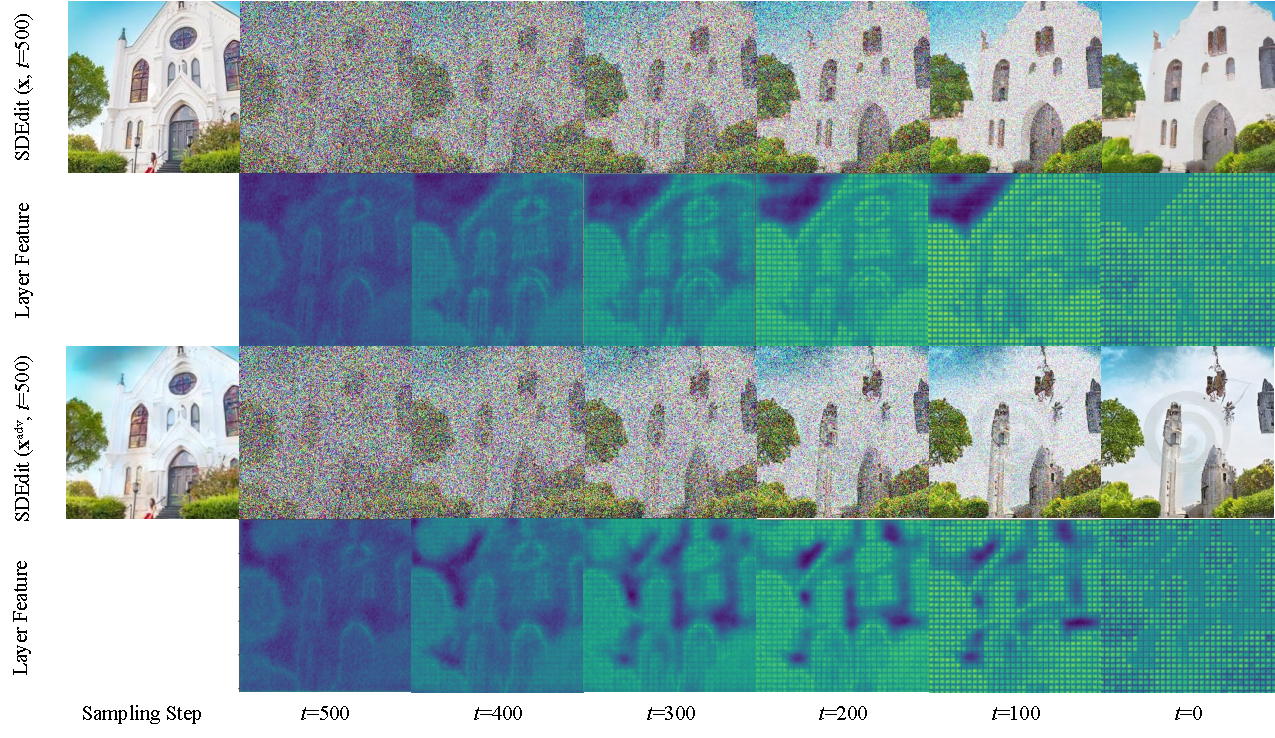
\includegraphics[width=0.9\linewidth]{figures/feature_visulization.pdf}
\caption{Qualitative example of corrupting feature representations in UNet: as the denoising process proceeds, the similarity of the feature map decreases, suggesting the representation is corrupted.}
\label{fig:feature_visulization}
\end{figure*}

\subsection{Qualitative Results of Loss Ablation}
Figure~\ref{fig:loss_ablation} presents qualitative results of loss ablation where i., ii., and iii. indicate performing PGAscent with different configurations. i. utilizes only semantic loss; ii. utilizes semantic loss with our latent optimization strategy; iii. utilizes both semantic loss, our proposed $\mathcal{L}_\text{fidelity}$ and latent optimization. The results show that our $\mathcal{L}_\text{fidelity}$ and latent optimization can enhance the adversarial image quality of PGAscent. Moreover, comparing our proposed two methods, AtkPDM$^+$ generates a more natural adversarial image than AtkPDM while maintaining attack effectiveness.

\begin{figure*}[h]
\centering
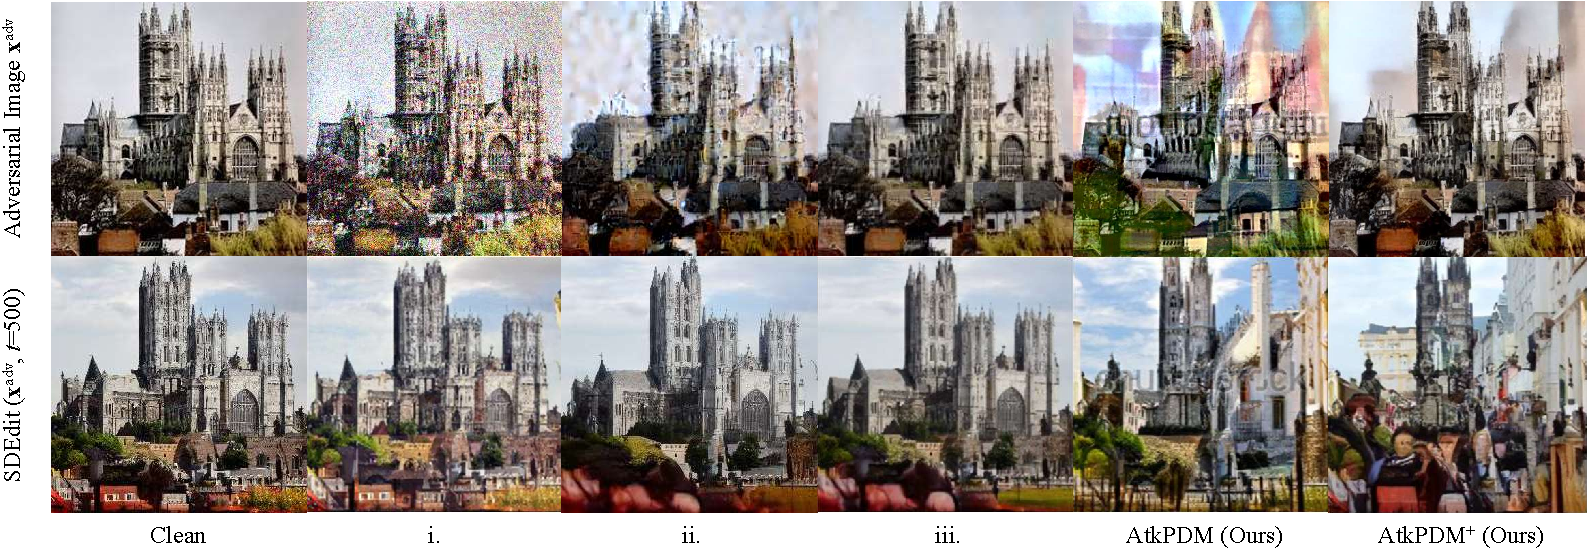
\includegraphics[width=1\linewidth]{figures/loss_ablation.pdf}
\caption{Qualitative example of different loss configurations. i. only semantic loss; ii. semantic loss and latent optimization; iii. semantic loss, $\mathcal{L}_\text{fidelity}$ and latent optimization.}
\label{fig:loss_ablation}
\end{figure*}

\subsection{Different Forward Time-step Sampling}

When using Monte Carlo sampling for optimization, the forward time step $t^*$ is sampled uniformly. We study the scenario that when $t^*$ is fixed for optimization. As shown in Figure~\ref{fig:different_timestep}, a primary result shows that when attacking $t^*=400$ to $t^*=500$, the attacking effectiveness is better than other time steps. In practice, we can not know user-specified $t^*$ for editing in advance; however, this suggests that diffusion models have a potential temporal vulnerability that can be further exploited to increase efficiency.

\begin{figure*}[h]
\centering
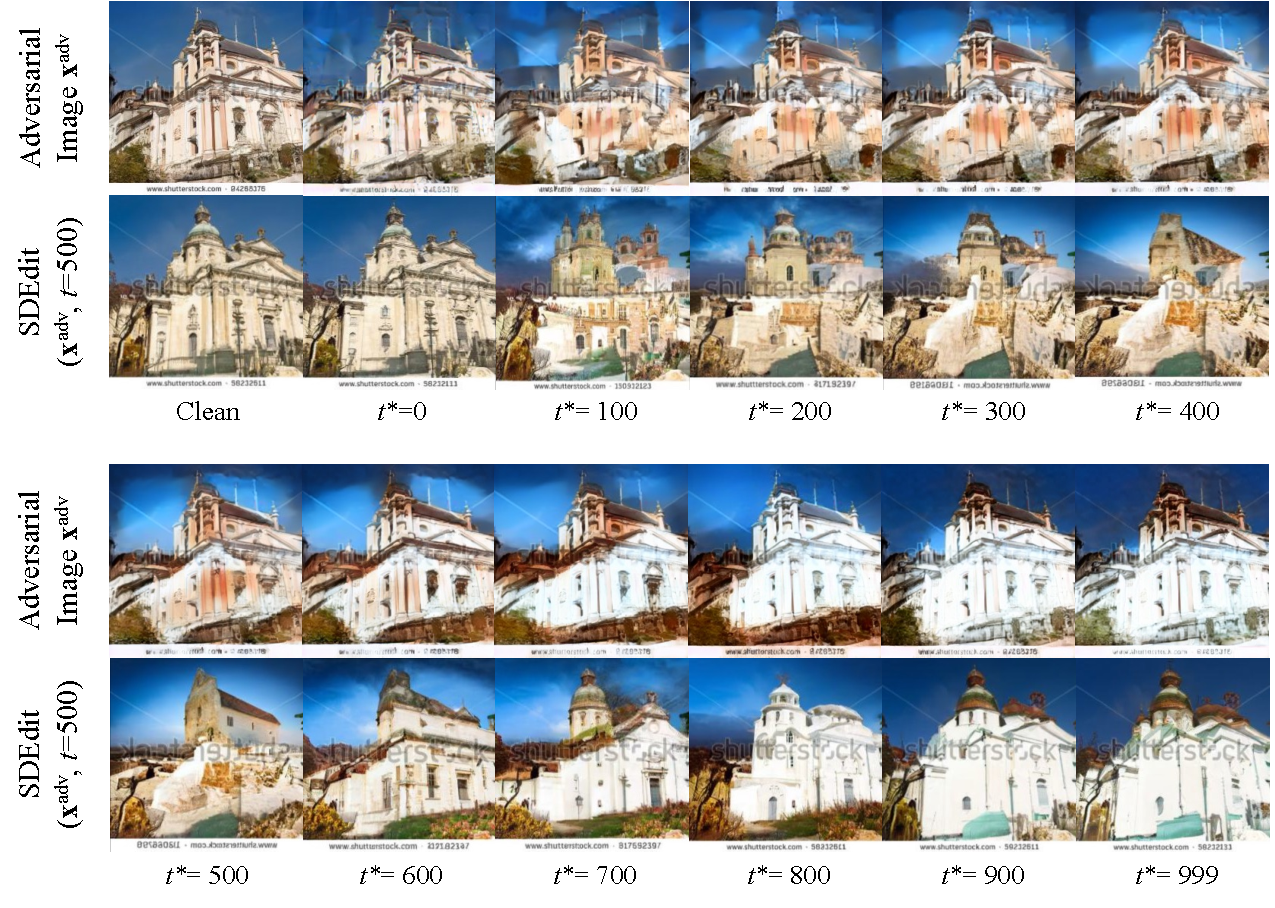
\includegraphics[width=0.9\linewidth]{figures/different_timestep.pdf}
\caption{Qualitative results of optimizing different fixed diffusion forward steps.}
\label{fig:different_timestep}
\end{figure*}

\subsection{More Qualitative Results}
We provide more qualitative results in Figure~\ref{supp:qualitative} to showcase that our method can significantly change or corrupt the generated results with little modification on adversarial images. In contrast, previous methods add obvious perturbation to adversarial images but still fail to change the edited results to achieve the safeguarding goal.

\begin{figure*}
\centering
\begin{subfigure}{1\linewidth}
    \centering
    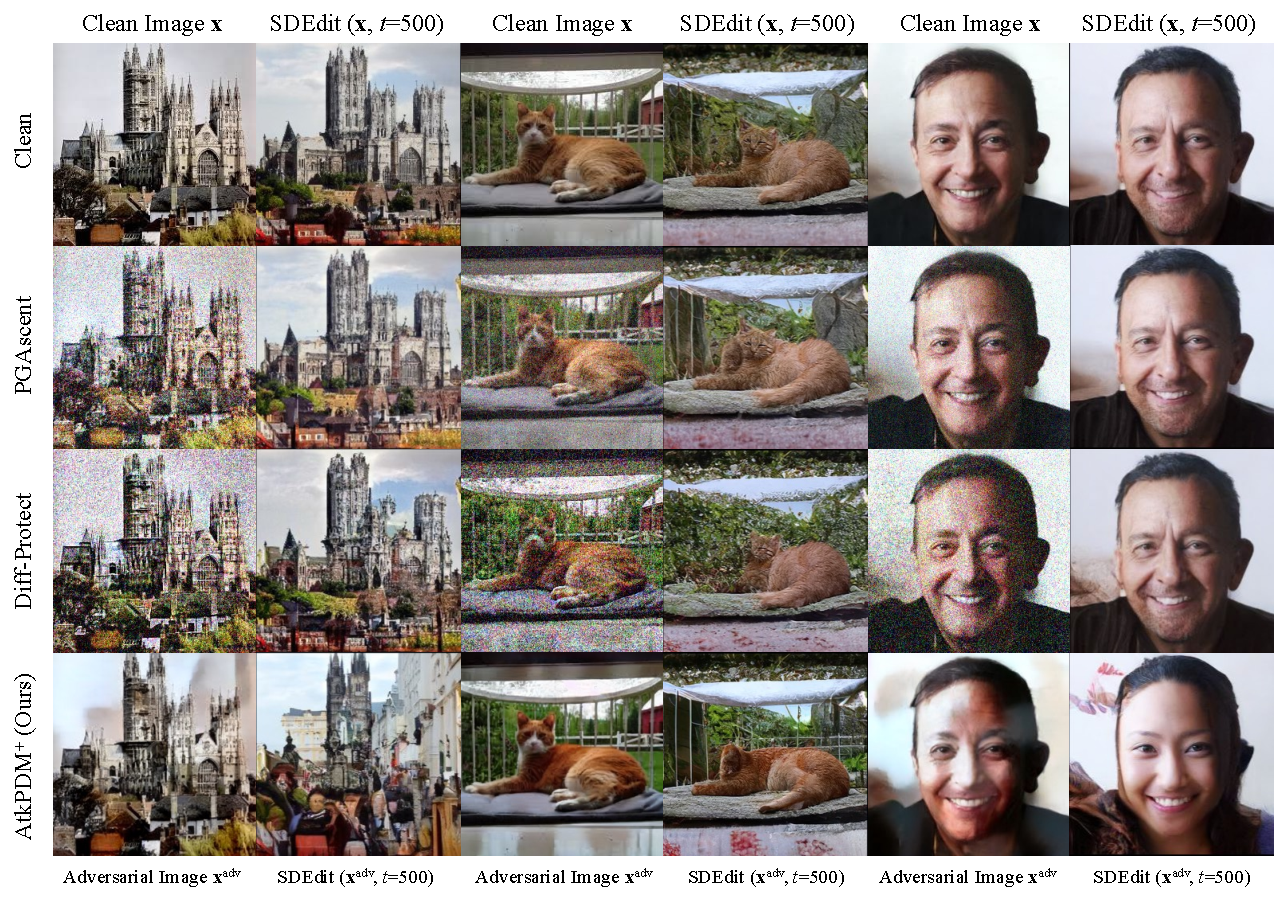
\includegraphics[width=0.9\linewidth]{figures/qualitative_results_1.pdf}
    \label{fig:qualitative_results_1}
\end{subfigure}

\begin{subfigure}{0.9\linewidth}
    \centering
    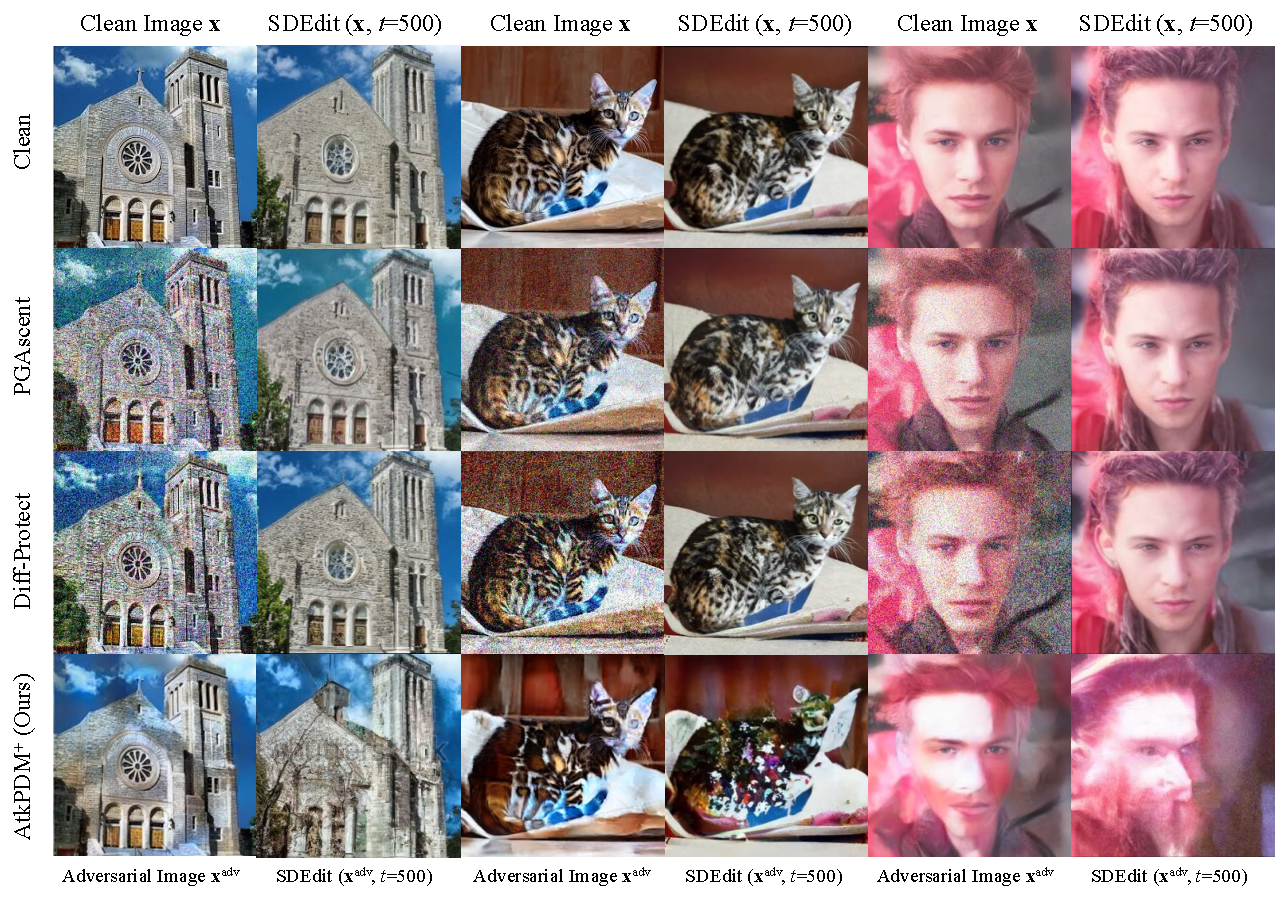
\includegraphics[width=1\linewidth]{figures/qualitative_results_2.pdf}
    \label{fig:qualitative_results_2}
\end{subfigure}
\caption{Qualitative results compared to previous methods: our adversarial images can effectively corrupt the edited results without significant fidelity decrease. The same column shares the same random seed for fair comparison.}
\label{supp:qualitative}
\end{figure*}

\subsection{Example of Loss Curves}

Figure \ref{supp:loss_curve} shows an example of our loss trends among optimization steps. $\mathcal{L}_\text{attack}$ has decreasing trend as the optimization step increases. $\mathcal{L}_\text{fidelity}$ has an increasing trend and converges to satisfy the constraint of the attack budget $\delta$.

\section{Limitations}
While our method can deliver acceptable attacks on PDMs, its visual quality is still not directly comparable to the results achieved on LDMs, indicating room for further improvement. More generalized PDM attacks should be further explored. 

\section{Societal Impacts}
Our work will not raise potential concerns about diffusion model abuses. Our work is dedicated to addressing these issues by safeguarding images from being infringed.

\begin{figure*}
\centering
\begin{subfigure}{1\linewidth}
    \centering
    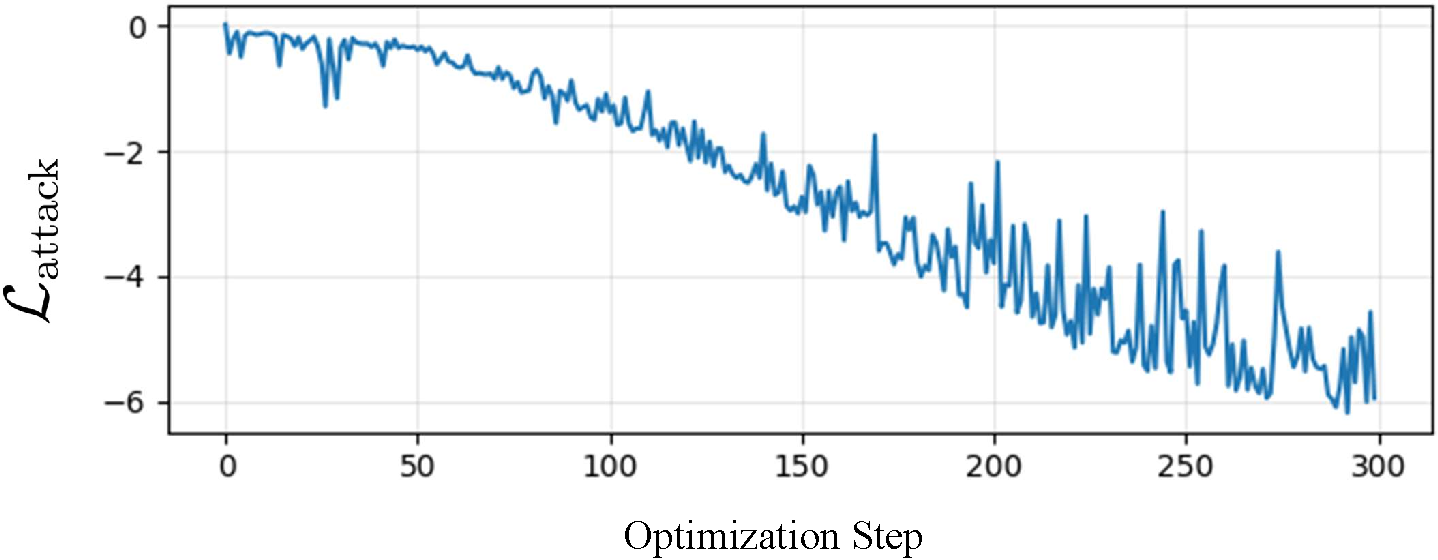
\includegraphics[width=0.7\linewidth]{figures/attack_loss_curve.pdf}
    \label{fig:attack_loss_curve}
\end{subfigure}

\begin{subfigure}{1\linewidth}
    \centering
    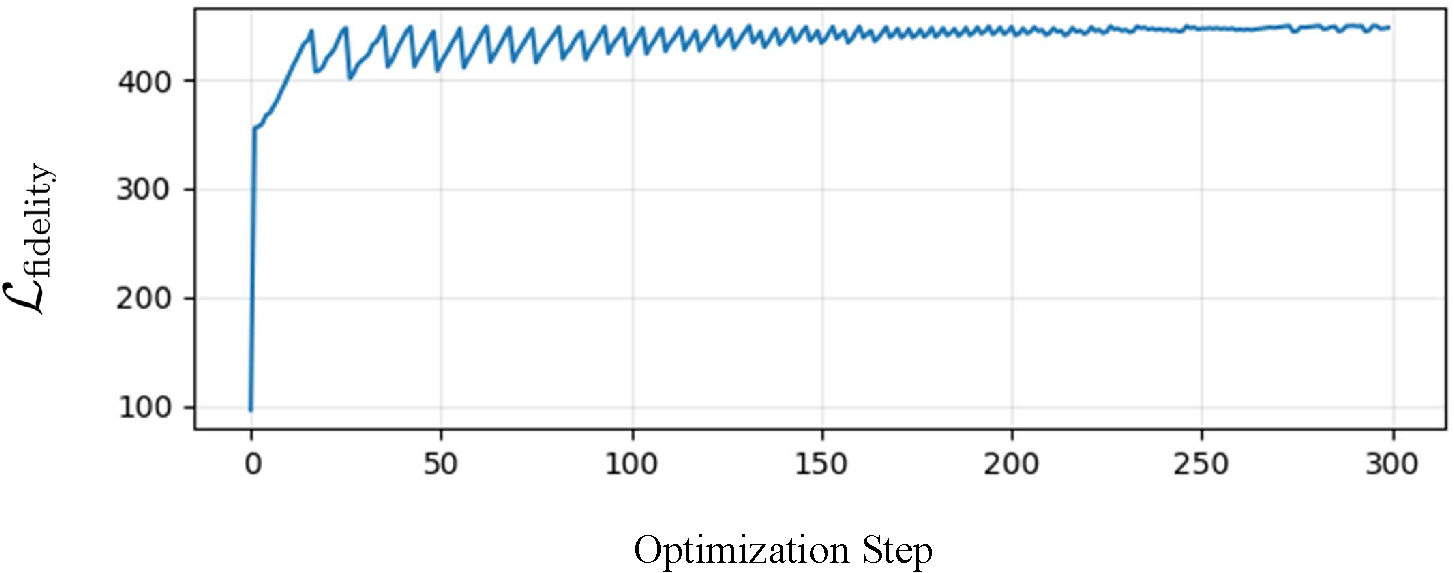
\includegraphics[width=0.7\linewidth]{figures/fidelity_loss_curve.pdf}
    \label{fig:fidelity_loss_curve}
\end{subfigure}
\caption{Loss curves of our $\mathcal{L}_\text{attack}$ and $\mathcal{L}_\text{fidelity}$ against optimization step.}
\label{supp:loss_curve}
\end{figure*}

\section{Details of Our Proposed Algorithm}

\subsection{AtkPDM Algorithm without Latent Optimization}

\begin{algorithm}[H]
    \caption{AtkPDM}
    \label{alg:attdpm}
    \small{
    \begin{algorithmic}[1] 
        \STATE{\textbf{Input:}
        Image to be protected $\mathbf{x}$, attack budget $\delta > 0$, and step size $\gamma_1, \gamma_2>0$}
        \STATE{\textbf{Initialization:} $\mathbf{x}^{\adv} \leftarrow \mathbf{x}$, $L_\text{attack} \leftarrow \infty$}
        \WHILE{$L_\text{attack}$ not convergent}
            \STATE{Sample timestep: $t \sim [0, T]$}
            \STATE{Sample noise: $\epsilon_1, \epsilon_2 \sim \normaldist$}
            \STATE{Compute original noisy sample: $\mathbf{x}_t \leftarrow \mathcal{F}(\mathbf{x}, t, \epsilon_1)$}
            \STATE{Compute adversarial noisy sample: $\mathbf{x}^{\adv}_t \leftarrow \mathcal{F}(\mathbf{x}^{\adv}, t, \epsilon_2)$}
            \STATE{Update $\mathbf{x}^{\adv}$ by Gradient Descent: \\
            $\mathbf{x}^{\adv} \leftarrow \mathbf{x}^{\adv} -
            \gamma_1 \sign(\nabla_{\mathbf{x}^{\adv}} \mathcal{L}_\text{attack}(\mathbf{x}^{\adv}_t, {\mathbf{x}_t}))$}            \WHILE{$\mathcal{L}_\text{fidelity}(\mathbf{x}^{\adv}, \mathbf{x}) > \delta$}
            \STATE{$\mathbf{x}^{\adv} \leftarrow \mathbf{x}^{\adv} -
            \gamma_2 \nabla_{\mathbf{x}^{\adv}} \mathcal{L}_\text{fidelity}(\mathbf{x}^{\adv}, \mathbf{x})$}
            \ENDWHILE
        \ENDWHILE
        \RETURN {$\mathbf{x}^{\adv}$}
    \end{algorithmic}
    }
\end{algorithm}


\subsection{2-Wasserstein Distance Between Two Normal Distribution}
Consider the normal distributions $\mathcal{N}_t:=\mathcal{N}(\mu_t, \Sigma_t)$ and $\mathcal{N}_t^{\adv}:=\mathcal{N}(\mu_t^{\adv}, \Sigma_t^{\adv})$. Let $\Pi(\mathcal{N}_t, \mathcal{N}_t^{\adv})$ denote a joint distribution over the product space $\mathbb{R}^n \times \mathbb{R}^n$. The 2-Wasserstein distance between $\mathcal{N}_t$ and $\mathcal{N}_t^{\adv}$ is defined as:
\begin{align*}
    \mathcal{W}_2^2(\mathcal{N}_t, \mathcal{N}_t^{\adv})
    =\min_{\pi \in \Pi(\mathcal{N}_t, \mathcal{N}_t^{\adv})} \int \|\mathbf{x}_t-\mathbf{x}_t^{\adv}\|_2^2 \text{d}\pi(\mathbf{x}_t, \mathbf{x}_t^{\adv}).
\end{align*}

Using properties of the mean and covariance, we have the following identities:
\begin{align*}
    &\int \|\mu_t-\mu_t^{\adv}\|_2^2 \text{d}\pi(\mathbf{x}_t, \mathbf{x}_t^{\adv}) = \|\mu_t-\mu_t^{\adv}\|_2^2, \\
    &\int \|\mathbf{x}_t-\mu_t\|_2^2 \text{d}\pi(\mathbf{x}_t, \mathbf{x}_t^{\adv}) = \trac(\Sigma_t), \\
    &\int \|\mathbf{x}_t^{\adv}-\mu_t^{\adv}\|_2^2 \text{d}\pi(\mathbf{x}_t, \mathbf{x}_t^{\adv}) = \trac(\Sigma_t^{\adv}), \\
    &\int (\mathbf{x}_t-\mu_t)^\top(\mathbf{x}_t^{\adv}-\mu_t^{\adv}) \text{d}\pi(\mathbf{x}_t, \mathbf{x}_t^{\adv}) \\
    &=\trac\left(\mathbb{E}[(\mathbf{x}_t-\mu_t)(\mathbf{x}_t^{\adv}-\mu_t^{\adv})^\top\right).
\end{align*}
Thus, the 2-Wasserstein distance can be expressed as:
\begin{equation}
\begin{aligned}
    \mathcal{W}_2^2(\mathcal{N}_t, \mathcal{N}_t^{\adv})
    &=\|\mu_t-\mu_t^{\adv}\|_2^2 \\
    + \trac{(\Sigma_t)} &+ \trac{(\Sigma_t^{\adv})}
    -2\max_{J \succeq 0} \trac(C),
\end{aligned}
\end{equation}
where $J$ is the joint covariance matrix of $\mathcal{N}_t$ and $\mathcal{N}_t^{\adv}$, defined as:
\begin{align*}
J = \left[
\begin{array}{cc}
    \Sigma_t & C \\
    C^\top   & \Sigma_t^{\adv}
\end{array}
\right],
\end{align*}
and $C$ is the covariance matrix between $\mathcal{N}_t$ and $\mathcal{N}_t^{\adv}$:
\begin{align*}
C = \mathbb{E}
\left[
(\mathbf{x}_t-\mu_t)(\mathbf{x}_t^{\adv}-\mu_t^{\adv})^{\top}
\right].
\end{align*}

By the Schur complement, the problem can be formulated as a semi-definite programming (SDP) problem:
\begin{equation}
\begin{aligned}
&\text{maximum} \quad \trac(C), \\
&\text{subject to } \quad
\Sigma_t - C^\top (\Sigma_t^{\adv})^{-1} C \succeq 0.
\end{aligned}
\end{equation}
The closed-form solution for $C$ derived from the SDP is:
\begin{equation*}
    C=
    \Sigma_t^{\frac{1}{2}}
    (\Sigma_t^{\frac{1}{2}}\Sigma_t^{\adv}\Sigma_t^{\frac{1}{2}})^\frac{1}{2}
    \Sigma_t^{-\frac{1}{2}}.
\end{equation*}

Finally, the closed-form solution for the 2-Wasserstein distance between the two normal distributions is given by:
\begin{equation}
\begin{aligned}
    \mathcal{W}_2^2(\mathcal{N}_t, \mathcal{N}_t^{\adv})
    &=\|\mu_t-\mu_t^{\adv}\|_2^2 \\
    + \trac{(\Sigma_t)} &+ \trac{(\Sigma_t^{\adv})}
    -2(\Sigma_t^{\frac{1}{2}}\Sigma_t^{\adv}\Sigma_t^{\frac{1}{2}})^\frac{1}{2}.
\end{aligned}
\end{equation}


\subsection{Alternating Optimization}
Let $\mathbf{y} = \mathbf{x}^{\adv}$, by Lagrange relaxation \cite{liu2023instruct2attack}, the objective function can be expressed as:    
\begin{equation}
F(\mathbf{x}, \mathbf{y}) = F_1(\mathbf{x}, \mathbf{y}) + \lambda F_2(\mathbf{x}, \mathbf{y}),
\end{equation}
where $\lambda > 0$ is the Lagrange multiplier and $F_1$, $F_2$ are defined as
\begin{align}
    F_1(\mathbf{x}, \mathbf{y})
    &=\mathcal{L}_\text{attack}(
    \mathcal{F}(\mathbf{x}, t, \epsilon_1), \mathcal{F}(\mathbf{y}, t, \epsilon_2)), \\
    F_2(\mathbf{x}, \mathbf{y})
    &=\max (\epsilon-\mathcal{L}_\text{fidelity}(\mathbf{x}, \mathbf{y}), \mathbf{0}).
\end{align}

The optimization is carried out in an alternating manner as follows:
\begin{align}
    & \mathbf{y}^{i+\frac{1}{2}} = \argmin_{\mathbf{y}} \left(F_1(\mathbf{x}, \mathbf{y}) + \lambda F_2(\mathbf{x}, \mathbf{y}^{i})\right), \label{eq:F1} \\
    & \mathbf{y}^{i+1} = \argmin_{\mathbf{y}} \left(F_1(\mathbf{x}, \mathbf{y}^{i+\frac{1}{2}}) + \lambda F_2(\mathbf{x}, \mathbf{y})\right). \label{eq:F2}
\end{align}

To solve Equation \ref{eq:F1}, we employ the Fast Gradient Sign Method (FGSM) \cite{ian2015fgsm}. The update is given by:
\begin{equation}
\mathbf{y}^{i+1/2} = \mathbf{y}^{i} - \gamma_1 \sign\left(\nabla_{\mathbf{y}^i} F_1(\mathbf{x}, \mathbf{y}^i)\right),
\end{equation}

For Equation \ref{eq:F2}, we utilize Gradient Descent, resulting in the following update:
\begin{align}
\mathbf{y}^{i+1} = \mathbf{y}^{i+\frac{1}{2}} - \Tilde{\gamma}_2 \nabla_{\mathbf{y}^{i+\frac{1}{2}}} \lambda F_2(\mathbf{x}, \mathbf{y}^{i+\frac{1}{2}}) \\
= \mathbf{y}^{i+\frac{1}{2}} - \gamma_2 \nabla_{\mathbf{y}^{i+\frac{1}{2}}} F_2(\mathbf{x}, \mathbf{y}^{i+\frac{1}{2}}).
\end{align}
Note that the gradient of $F_2$ can be derived as follows:
\begin{align*}
    \nabla_{\mathbf{y}} F_2(\mathbf{x}, \mathbf{y})
    = \mathbb{I}_\mathcal{C'} \odot
    \nabla_{\mathbf{x}^{\adv}_t} \mathcal{L}_\text{fidelity}(\mathbf{x}, \mathbf{y}),
\end{align*}
where $\mathbb{I}_\mathcal{C'}$ is indicator function with constraint $\mathcal{C} = {\{\mathbf{y} \in \mathcal{M} \mid \mathcal{L}_\text{fidelity}(\mathbf{x}, \mathbf{y}) \leq \epsilon\}}$.\\

Please note that after references, we also provide more results presented in Figures~\ref{fig:loss_ablation}, ~\ref{fig:different_timestep}, ~\ref{supp:qualitative}, and~\ref{supp:loss_curve}, please refer to subsequent pages.



\end{document}
